\documentclass[acmsmall,table,xcdraw]{acmart}


\usepackage{xcolor}
\usepackage{cite}
\usepackage{amsmath,amssymb,amsfonts}
\usepackage{algorithmic}
\usepackage{textcomp}
\usepackage{float}
\usepackage{threeparttable}
\usepackage{amsmath}
\usepackage{enumitem}
\usepackage{graphicx}
\usepackage{mathtools,cuted}
\usepackage{tablefootnote}
% \usepackage{xcolor}
\usepackage{lipsum}
\usepackage{subcaption}
\usepackage{multirow}
\usepackage{longfbox}
\usepackage{makecell}
\usepackage{longtable}


\DeclarePairedDelimiter\abs{\lvert}{\rvert}
\newcommand{\topicquote}[1]{\\ \hspace*{2em}\emph{``#1"}}


\title{
Understanding the Growth and Challenges of New Programming Languages: An Empirical Analysis
}


% \author{Partha Chakraborty}
% \affiliation{%
%   \institution{Bangladesh University of Engineering and Technology}
%   \department{Department of Computer Science and Engineering}
%   \city{Dhaka}
%   \country{Bangladesh}
% }
% \email{shuvopartho@gmail.com}

% \author{Rifat Shahriyar}
% \affiliation{%
%   \institution{Bangladesh University of Engineering and Technology}
%   \department{Department of Computer Science and Engineering}
%   \city{Dhaka}
%   \country{Bangladesh}
% }
% \email{rifat@cse.buet.ac.bd}

% \author{Anindya Iqbal}
% \affiliation{%
%   \institution{Bangladesh University of Engineering and Technology}
%   \department{Department of Computer Science and Engineering}
%   \city{Dhaka}
%   \country{Bangladesh}
% }
% \email{anindya@cse.buet.ac.bd}




\acmJournal{TMIS}
\citestyle{acmauthoryear}
\begin{document}

\newcommand{\rcomment}[1] { \textcolor{red}{#1}}
\newcommand{\boxtext}[1]{\begin{longfbox}#1\end{longfbox}}
\newcommand{\eqrow}[1]{
    \vbox{
        \begin{equation}
            \nonumber
            \begin{split}
                #1 \hspace{10em}
            \end{split}
        \end{equation}
        } \\
     }
% \thispagestyle{empty}
% \pagestyle{empty}

\begin{abstract}
New programming languages (e.g., Swift, Go, Rust, etc.) are being introduced to provide a better opportunity to developers by matching the requirements of new platforms and application contexts. In the beginning, a programming language is likely to have constraints of resources that encourage the developers to seek help from experienced peers active in Question-answering (QA) sites such as Stack Overflow (SO). In this study, we would like to analyze the discussions on three popular new languages that are introduced after the inception of SO (2008) and also match those with the relevant activities in GitHub whenever appropriate. The relevant posts in SO present an interesting representation of the growth/evolution of that language and also, expose the demands of the relevant development community. The major findings of the study are: (i) the difficult topics of new languages are quite common, (ii) the time when adequate resources are expected to be available vary from language to language, (iii) the unanswered question ratio increases regardless of the age of the language, (iv) a new language is benefited from its predecessor language and (v) there is a relationship between developers' activity pattern and growth of the language. The study outcome is likely to help the owner/sponsor of these languages to design better features and documentation and software developers or students to prepare themselves to work on these languages in an informed  .
\end{abstract}
\maketitle

\section{Introduction}
\label{sec:introduction}
After the release of a new programming language, it takes time for the developers to get acquainted with that language. The developers who work on the new languages are likely to face problems that are similar to the solved problems of mature languages. Detailed knowledge of the growth of resources of a new language can help prevent these issues from appearing again for another language. Moreover, earlier releases of new languages often contain bugs. Developers of the new languages often feel the absence of a library or feature that has already been available in other languages. It is also possible that low-quality documentation and absence of resources in question-answer (QA) sites make the skill growth of developers of new languages slower.

\iffalse
To better help developers of new languages, it is imperative to know how the resources of a language build up in QA site, the impact of language bug in software development and the effects of the absence of a feature. The quality of the support provided in the early stages plays a pivotal role in the acceptance of the language. Despite that, we often notice the absence of quality support for new languages in starting years. To fill the gap in support, language owners can offer extensive support period for new languages, but this is not the only factor contributing to the growth of languages. Identification of all the factors contributing to the growth of language may help to build a collaborative model to support the growth of new languages. In addition to helping the developers, this type of study will help language designers in selecting features, designing documentation and also determining extending support period for developers.
\fi 

To make software development easy, maintainable, robust, and performance-guaranteed, new programming languages are being introduced. For example, Swift was introduced in June 2014 as an alternative to Objective-C to achieve better performance in all the aspects mentioned above. At the initial stage of its lifetime, a programming language is likely to have constraints of resources, and consequently, developers using these languages face additional challenges. Naturally, the developers seek help from community experts of question-answering (QA) sites such as Stack Overflow (SO). Hence, it is expected that the discussions on issues related to a new language in SO represents the growth of that language and also exposes the demands of the development community who use that language. 

To the best of our knowledge, there is yet to be any Software Engineering research that focuses on the specific characteristics of the new languages by mining relevant discussions from SO. In this study, we would like to fill this gap analyzing the discussions on Swift, Go, and Rust that were the most popular languages introduced after the inception of SO (2008). Hence, the evolution right from the beginning of these languages is expected to be reflected in SO. From now on, by the \emph{new language},  we imply Swift, Go and Rust languages. We also match the SO discussions with the relevant activities in GitHub whenever appropriate. 

The primary objective of this research is to study different characteristics of the discussions in SO relevant to these new languages and observe their journey towards maturity. On this goal, our specific research questions are as follows.
\begin{itemize}
\item \textbf{RQ1.} What are the difficult topics in the questions of new languages in Stack Overflow?
\item \textbf{RQ2.} When can we expect the availability of adequate resource of the new languages in Stack Overflow?
\item \textbf{RQ3.} Is there any relation between the growth of a language and developers' activity pattern of that language?
\item \textbf{RQ4.} What are the characteristics of answer pattern for new languages in Stack Overflow?
\item \textbf{RQ5.} Are the questions of new languages in Stack Overflow answered mostly by the developers of predecessor languages?
\end{itemize}

The motivation behind investigating the first research questions is to help the owner/sponsor of these languages to design better features and documentation which would eventually benefit the developers. The general software developers or students can receive insight into how to prepare themselves to work on these languages. Moreover, the last three research questions would cater to the academic interest of researchers by presenting interesting parameters of evolution pattern of new languages and their reflection in SO.


The major findings of the study are: (i) (i) the difficult topics of new languages are quite common, (ii) the time when adequate resources are expected to be available vary from language to language, (iii) the unanswered question ratio increases regardless of the age of the language, (iv) a new language is benefited from its predecessor language and (v) there is a relationship between developers' activity pattern and growth of the language.


\section{Related Works}
\label{sec:Related Works}
There have been many works on Stack Overflow data, analyzing trends and characteristics. Barua et al.\citep{Barua2012} have investigated the question ``What developers are asking?" in their work.
Rosen and Shihab\citep{Rosen2015} had a similar work focusing on mobile developers while Bajaj et al.\citep{Bajaj2014}  focused on web developers.

Hart and Sharma\citep{Hart2014} had suggested considering user reputation, the social reputation of answerer and post length to judge post quality.

Reboucas et al.\citep{Reboucas2016} have compared the data from Stack Overflow with opinions of 12 Swift developers to answer three research questions - common problems faced by Swift developers, problems faced by developers in the usage of `optionals,' and error handling in Swift. They used Latent Dirichlet Allocation (LDA) to identify the topics from questions of Stack Overflow and then cross-checked the findings by interviewing Swift developers. These are different from our research questions.

Zagalsky et al.\citep{Zagalsky2016} have analyzed the R language using data from both Stack Overflow and R-help mailing list. They focused on the participation pattern of users in the two communities. They collected user information who are active in both sites and later mining on their activities (questions, answers) they tried to answer how communities create, share and curates knowledge. Vasilescu et al.\citep{Vasilescu2014} have compared popularity and user activity level between StackOverflow and R-help mailing list. They followed a similar approach like Zagalsky et al.\citep{Zagalsky2016} by identifying active users in both communities. They have some interesting finding on the decreasing popularity of mailing list and influence of reputation system in Stack Overflow. Their work is mainly focused on identifying user behavior of these communities.

Tausczik et al.\citep{TausczikWC17} measured the effect of crowd size on Stack-Exchange question quality. They have found that among question audience size, contributor audience size and topic audience size, contributor audience size has a higher effect on solution quality. They have classified the problems into three problems: error problems, how to problems and conceptual problems. Error problems are very specific, as a result, no matter how much the audience size is 25\% problems are never solved. Large audience provides a diverse solution which is critical for how to problems. Conceptual problems are trickier and rarely solved with a small audience.

Srba et al.\citep{Srba2016} had discussed the reason behind the increasing failure and churn rate of Stack Overflow. In their work, criticizing the existing automatic deletion and classification of posts, they introduced a new reputation system. They also suggested to follow answer oriented approach instead of the current asker-oriented approach. Instead of focusing on the highly expert users, Stack Overflow should engage users of all levels.
\section{Research Setting}
\label{sec:Research Setting}
This section introduces four research questions along with the motivation for this question. In this section, we will describe the research questions.

\subsection{Research Questions}
\noindent \textbf{RQ1.} What are the difficult topics in the questions of new languages in Stack Overflow?

\indent  Developers of new languages face problems that are rarely answered or get \emph{delayed answers}. By the \emph{delayed answer}, we imply that answer which is accepted by the user and received after the median answer interval of that month. We want to know about these questions so that special measures can be taken to answer this question.

\noindent  \textbf{RQ2.} When can we expect the availability of adequate resource of the new languages in Stack Overflow?

\indent After the introduction of a new language, the resources of those languages may be absent in QA sites. Gradually the lackings will be met. We want to know the time interval after which we can expect the availability of these resources of new languages in Stack Overflow at a satisfactory level.

\noindent  \textbf{RQ3.} Is there any relation between the growth of a language and developers' activity pattern of that language?

\indent Stack Overflow has become one of the most prominent QA sites over the years. It has been used as a source to gain insight into developers' activity\citep{Ahmed2017}. We can observe developers' activity from the frequency of question and answer in Stack Overflow and also from the number of developers and repositories of that language in GitHub. GitHub provides \emph{issue}\citep{GithubIssue} to keep track of task, bug and feature request for a project. Most of the issues of a GitHub project are associated with bugs or feature request\citep{Bissyande2013}. Therefore, it can be assumed that the solution to the issues leads to the advancement of the project. Hence, issues reflect the growth of the project. Moreover, every new release of a language implies the growth of that language. Thus, developers activity pattern after a new release of that language can also help to understand the relationship. We want to understand the relation between the growth of a programming language and developers' activity pattern.

\noindent  \textbf{RQ4.} What are the characteristics of answer pattern for new languages in Stack Overflow?

\indent With the evolution of a new language, the number of skilled developers increases. Being the most used programming related QA site, Stack Overflow is supposed to reflect that change. The increasing number of skilled developers may have its impact on answer patterns such as the expected interval of first and accepted answers, unanswered question ratio. By answer interval, we imply the delay between a question posted and an answer received. We want to know the characteristics of the answer pattern of new languages.

\noindent  \textbf{RQ5.} Are the questions of new languages in Stack Overflow answered mostly by the developers of predecessor languages?

\indent Stack Overflow includes developers from a diverse domain. We are interested to see if there is a pattern that the experts in the predecessor of a new language mostly answers the questions of that language (e.g., Objective-C for Swift).

\iffalse


\noindent  \textbf{RQ6.} Is there any change over time in topics of Stack Overflow questions with the growth of the relevant language?

\indent Evolution of a language has many phases. These phases must have their footprint in the topics of the questions asked by the developers of the new languages. Hence, we want to know the topics of the questions asked by developers with respect to a timeline so that we can identify those phases.

\noindent \textbf{RQ7:} \emph{How do developers respond to the release of a new version of a language?}

\indent A new release of a language comes with a new and updated feature set. These updated or new features must have some impact over developer community. It may trigger new thread of question in Stack Overflow. We want to know the after effect of such release.
\fi

\section{Methodology}
\label{sec:dataset preparation}
The following steps are followed to develop the dataset for this study.

\begin{enumerate}
    \item \textbf{Download Stack Overflow dataset:} For our analysis, we have collected the December 2017 Stack Overflow data dump which is available in the Stack Exchange data dump. In Stack Overflow schema, both question and answer are considered as \emph{post}. The post table of the data dump contains all the information of a post like a title, tags, body, creation date, view count, type (question or answer) and accepted answer identifier. An answer is accepted if the questioner marks that answer as accepted. Our dataset includes 4,17,82,536 questions and answers posted over some time of over 9 years from August 2008 to December 2017 by 39,40,962 users of Stack Overflow. Among these posts 1,63,89,567 (39\%) are questions and 2,52,97,926 (61\%) are answers of which 87,04,031 (21\%) are marked as accepted answers.
    
 
    \item \textbf{Develop tag set:} To compare the growth of languages, we have to separate the posts by language. Posts on Stack Overflow can be about any topic, we need a way to identify posts by language. Every Stack Overflow post is associated with at least one tag. We consider a post is associated with one of the new languages if that contain at least one tag of tag set of that respective language. We have created an initial set of tag $\uptau_0$ for each language by manually inspecting the tag table of Stack Overflow schema. Next, we go through the Stack Overflow dataset $\mathcal{S}$ and extract questions $\rho$ whose tags contain a tag from  $\uptau_0$. Third, we extract tags of the posts in $\uprho$ to form the set of candidate concurrency tags $\uptau$. Now we have a set of tag $\uprho$ for each language which includes all tags of that language.However, set $\uprho$ may include tags which may be irrelevant to new languages. So following the  approach of Rosen et al.\citep{Rosen2015} we have  used two heuristics $\alpha$ and $\beta$ to find the the significantly relevant tags for each language. 
    
    \begin{equation}
        \alpha = \dfrac{number \ of \ posts \ with \ tag \ t \ in \ \uprho}{number \ of \ posts \ with \ tag \ t \ in \ \mathcal{S}}
    \end{equation}
    \begin{equation}
         \beta = \dfrac{number \ of \ posts \ with \ tag \ t \ in \ \uprho}{number \ of \ posts \ in \ \uprho}
    \end{equation}

    We have experimented with a broad range of $\alpha$ and $\beta$  and found that $\alpha = 0.01$ and $\beta=0.01$ provides a significantly relevant set of tags. Relevant tags selected for this study is presented in appendix ~\ref{appendix:tagrelevance}.

% To compare the growth of languages, we have to separate the posts by language. Every Stack Overflow post is associated with at least one tag. We consider a post is associated with one of the new languages if that contain at least one tag of tag set of that respective language. To develop a set of tag for each language, we have used keywords to search in the tag table and then by manual inspection we have identified relevant tags for each language. 
    
    \item \textbf{Extract posts of new languages:} Using the tag set prepared in the previous step, we have separated the posts by language. We have 4,37,880 Swift posts, consisting of 1,88,065 (43\%) questions and 2,49,815 (57\%) answers of which 94,310 (21.6\%) are accepted answers. We have 72,843  Go posts, consisting of 30,286 (41.6\%) questions and 42,557 (58.4\%) answers of which 19,178 (26.3\%)  are accepted answers. We have 18,311 Rust posts, consisting of 8,083 (44.1\%) questions and 10,228 (55.9\%) answers of which 5,964 (32.6\%) are accepted answers. 

     \item \textbf{Data extraction from GitHub:} GitHub provides access to data of public repositories and users through API\footnote{https://developer.github.com/v3/}. The new languages have their official repository in GitHub. We have collected the creation date and closing date of the issues from the official repositories of these new languages. GitHub issues have two states `open' and `closed.' As soon as an issue is taken care of, it changes its state from `open' to `closed.' Along with the frequency of issues, we have also collected the states of issues. Besides, we have collected the number of users and repositories of each new language.
\end{enumerate}

\iffalse

 \item \textbf{Preprocessing of posts for topic modeling:} To avoid noise, we preprocess the post before topic modeling\citep{Barua2012}. First, all the codes enclosed in <code> tags, HTML tags, and url are removed. Second, the Porter stemming algorithm\citep{Porter1997} is applied to convert the words into their base form. Third, all the articles and stop words are removed. Now, the posts are ready for topic modeling. We have used MALLET's Latent Dirichlet Allocation (LDA)\citep{Blei2003} to infer topics automatically.
 
 
 
 Stack Overflow publishes its data periodically. We have collected the Stack Overflow data dump in  October 2018. There are total 38485046 posts(both question and answer) in that dump. Stack Overflow posts are associated with tags. Though the tags are added by the users, in the moderation process correct tags will be associated with that post. To separate the posts by languages, we rely on tags. We carefully curated a tag set for each of these languages based on keywords, frameworks etc. from the tag table of Stack Overflow.

GitHub provides access to public data of repository and user through API\footnote{\url{https://developer.github.com/v3/}}. By using that API we have collected information about the official Go, Rust and Swift repository, the number of users and number of repositories of each language.
\fi
\section{Result and analysis}
\label{sec:Results}
Now we present the result of our study and analogies for all the research questions.

\subsection{RQ1: Difficult topics of new languages}
\label{RQ1}

To answer this research question, we have considered \emph{less answered} questions. By \emph{less answered} question, we imply those questions that have no accepted answer or have an accepted answer but received after the median accepted answer interval of that month. \textcolor{green}{Accepted answer interval is the difference between the creation date of the accepted answer and the question. To identify less answered questions, first, the median of the accepted answer interval is calculated for each language. Second, questions that have no accepted answers, and questions whose accepted answer interval is greater than the median accepted answer interval of that language are collected. After accumulating these questions, we have performed LDA to identify the topics. LDA (Latent Dirichlet Allocation) is a generative statistical model. It assumed each document is a mixture of a small number of topics. We have tested multiple topic numbers in our dataset and found that ten topics per language are the best fit for our data. From LDA, we received multiple sets of tokens. Then by manually comparing the token set with the associated question, we identified the actual topic for each set. Keywords of the topics are presented in 
Table ~\ref{appendix:LDA topic} in Appendix.}
 
Difficult topics of Swift are presented below.
\begin{enumerate}
\item \textbf{UI:} UI allows for the interaction between software and its user. UI is the most significant topic for Swift based on Stack Overflow questions. UI questions includes questions like how to achieve this UI function?, how to use multiple UI component like button, audioplayer together? etc.
\topicquote{I have a UIImageView that allows a user ... how to place it in another UIImageView for display when the user pushes that button ...}

\item\textbf{View Controller lifecycle:} View controller is used to manage the app's interface. Questions related to the life cycle of this view controller belong to this category.
\topicquote{I am trying to set up a UIScrollView so that I can swipe between my view controllers ... I just want the whole screen to be a scroll view which allows me to swipe between my view controllers. How would I go about doing that?}

\item \textbf{Mutability:} Immutable variable allows developers to create a variable which will not change ever. It seems developers face problem in the syntax and use of the immutable variable.
\topicquote{I am trying to add an item to my array (which was declared as a var), using anything that might work (+=, append, insert), however, I keep getting the error 'Immutable value of type `AnyObject[]' only has mutating members named `append' ...}

\item \textbf{Data Handling:} It is apparent that Swift developers struggle to interact with video data. This category includes questions which seek for direction like how to save, stream or receive video from network.
\topicquote{I'm playing around with using AVFoundation in Swift Normally when I set up a video camera capture session, I do something like the ... I'm struggling to find how actually to get this working.}

\item \textbf{Migration problem:} Migration problems are two types . (1) The developer is migrating from another language (most of the case Objective-C) and facing problems to mimic the exact logic in Swift, (2) developer is migrating from an old project and facing problem in Xcode. 
\topicquote{I'm not sure if this is something to do with SWIFT or some bug, but I used to be able to call this in objective c ...}
\iffalse
\topicquote{I get this error after adding a Swift class to an old Xcode project. How can I make the project run again?}
\fi

\item \textbf{Documentation clarification:} This category includes questions which seek for the clarification of documentation of Swift itself or its' library.
\topicquote{The documentation I've found is terribly unclear on this - what I'd like to do is use the provided Xcode image library ...}

\iffalse
\textbf{Resource:} This category includes questions which are seeking proper direction and resource. It is apparent that Swift need resources in Swift game development.
\topicquote{I'm trying to replicate the Stanford Matchismo game from "Developing ios apps for iPhone and iPad" in iTunesU in Swift ... Has anyone figured out how to do this yet?  }
\fi
\end{enumerate}

Difficult topics of Go are presented below.
\begin{enumerate}

\item \textbf{Problem in using library:} GRAIL and GORM related problems are the most frequent and is part of this category. Though most of the problems are user specific, it seems they need proper attention.
\topicquote{The following Groovy code creates a GORM-persisted domain class called Foo when written to grails-app ... if I instead write ``public class Foo" the class does NOT get GORM-persisted, I'm running the latest stable release of Grails.}

\item \textbf{Serving request:} This category includes questions which are related to serving request and HTML files in Go language.
\topicquote{What website has some good, up to date resources on using Go HTML/templates, especially in regard to parsing HTML files...}

\item \textbf{Go channel:} Channels are typed conduit through which values can be sent or received. 
\topicquote{I'm very interested in the concurrency model of Google's Go programming language, with very lightweight goroutines and a system of communicating channels...is there an approximation of goroutines or go channels available for C++?}

\item \textbf{Compilation problem:} This category includes questions related to compilation problem. Go language requires a directory structure for compilation. It seems that the structure is not clear to developers.
\topicquote{I noticed the go/ast, go/token, go/parser, etc. packages in the src/pkg/go folder. However, the GCC compiler was based on C files located in src/cmd/gc. My question regards the new go command in Go that builds and runs programs: does this tool depend on the packages I referenced above?...}

\item \textbf{Memory:} Memory allocation and sharing between two separate programs in Go language belong to this category. 
\topicquote{I want to make an array of size N in go, but I don't know what N will be at compile time, how would I allocate memory for it?...}

\item \textbf{Migration problem:} The developers migrating to Go language often seek a solution with reference to the language they migrating from. It means developer expert in another language also faces hard times in Go. 
\topicquote{We want to rewrite kodingen.com backend with Go which currently is Java, running as a daemon using Jsvc. ... I have never touched any C in my life ... simple requirements give me hope that I can start using this wonderful language. What would you advise? Is C still better?}
\end{enumerate}

Difficult topics of Rust are presented below.
\begin{enumerate}

\item \textbf{Use of Struct:} Developers are struggling to get the exact behavior from Rust struct and in destructuring a struct.
\topicquote{I am trying to build a wrapper struct around the ... therefore I need to keep them around. How can I fix this structure? }

\item \textbf{Mutability:} A immutable variable is one which can not change its value after one assignment.
\topicquote{... I ran into trouble when I tried to return a closure that mutates a captured parameter ...}

\item \textbf{Parallel execution:}  Questions related to parallel execution belong to this category.
\topicquote{I am writing a Phoenix client library for Rust, taking advantage of the async WebSocket client from rust-websockets. Right now I am having trouble figuring out how to pass callback functions into the thread that is handling the web socket traffic ... }

\item \textbf{Borrow mechanism:} To access data without taking ownership over it, Rust uses a borrowing mechanism. Developers are facing to determine the scope and when to use it.
\topicquote{I tried to borrow a variable .... it is only saying out of scope }

\item \textbf{Use of Trait:} Rust trait is a collection of methods which can be implemented by any class to use those methods. Developers, especially new developers are facing a hard time to excel in Rust traits.
\topicquote{I'm trying to learn Rust, but I am faced with difficulty when I implement the trait for one of my types.}

\item \textbf{Migration problem:} Like the other two languages, developers migrating to Rust face problems in mimicking logic in Rust.
\topicquote{I am hoping to re-write some parts of a Python project in Rust to speed up things...I am capable of returning complex arrays/structures in Python. And this does not work properly in Rust.}

\iffalse
\item \textbf{Documentation clarification:} Developers often seek clarification about Rust documentation in Stack Overflow. 

\topicquote{I'm an absolute beginner to Rust and systems programming in general. ... I've only come across in C++, but never inline const types. Can someone please provide a beginner-friendly explanation of how this works? )}

\item \textbf{Portability of application:} After developing an application it needs to be delivered to the owners. Developers are facing problem in making portable application with all of their dependencies.

\topicquote{I have a dependency in my Cargo file that needs to be different by platform, specifically, the default features. Here's what I am trying to do ... But this doesn't seem to do what I want. On my Mac it appears to be using the bottom target line as if I just specified hyper = ``0.9". If I do cargo build as specified, I get errors with regard to openssl However, if I build it like this:Then it builds fine. This indicates to me that the cfg for "macos" isn't working while it works for other platform. How do I make this work, or more specifically, how do I solve the dependency which will work for all platforms.)}
\fi
\end{enumerate}

\begin{figure}[htbp]
\centering
\includegraphics[scale=0.35]{figures/TopicChart.eps}
\caption{Difficult topics of new languages}
\label{fig:less unaswered topics}
\end{figure}

Figure~\ref{fig:less unaswered topics} shows the top 5 difficult topics of new languages with their percentage. It is clear from the topics presented above that the developers of new languages face some problems regardless of the language. 
It is apparent that developers all the three languages face migration problems. 
Another common topic is documentation clarification. Developers ask this type of question as the documentation is not clear or ambiguous. 
% Please add the following required packages to your document preamble:
% \usepackage[table,xcdraw]{xcolor}
% If you use beamer only pass "xcolor=table" option, i.e. \documentclass[xcolor=table]{beamer}
\begin{table}[H]
\begin{tabular}{|l|l|l|}
\hline
Swift                                     & Go                                        & Rust                                      \\ \hline
UI                                        & Problem in using library                  & Use of Struct                             \\ \hline
View Controller lifecycle                 & Serving request                           & \cellcolor[HTML]{999903}Mutability        \\ \hline

\cellcolor[HTML]{999903}Mutability        & Go channel                                & Parallel execution                        \\ \hline
Data handling                             & Compilation problem                       & Borrow mechanism                          \\ \hline
\cellcolor[HTML]{4793A5}Migration Problem & Memory                                    & Use of Trait                              \\ \hline
Documentation clarification               & \cellcolor[HTML]{4793A5}Migration problem & \cellcolor[HTML]{4793A5}Migration problem \\ \hline
\end{tabular}
\caption{Difficult topics of new languages}
\label{table:language topics}
\end{table}
\textcolor{blue}{We presented a textual representation of Figure \ref{fig:less unaswered topics} in Table \ref{table:language topics}. It is noticeable that there are a few similarities among the topics. One common topic is the  \emph{migration problem}. Developers of the new languages try to migrate from the mature/old languages. Thus they request support regarding how to mimic the exact software behavior in a new language or query about equivalent library or syntax to another language. One interesting information visible from Figure \ref{fig:less unaswered topics} is that the occurrence of migration problems among difficult topics is quite low for Swift language. That might be due to its close linkage with Objective-C. Another common difficult topic is  \emph{mutability}. Swift and Go language developers often face difficulties in using the immutable feature. We have also observed that topics are related to the domain of the programming language. In Swift, we observed topics related to application development such as user interface, view controller, etc. For Go and Rust, we observed topics related to server-side development, such as request serving in a web server.}

\boxtext{\textbf{Finding 1:} In general, questions related to migration are common in new languages.}
\subsection{RQ3: Expected time of availability of adequate resources of new languages}
\label{RQ2}

It is hard to define ``adequate resource'' of a programming language in QA site. However, we can use an indirect approach to measure adequate resource. Two major types of Stack Overflow questions are \emph{repetitive} questions and the \emph{new} questions. By \emph{repetitive} question we mean the same question or same problem but the developers \citep{TausczikWC17} faced this problem in another platform or environment. The decrease in the number of the new question indicates that Stack Overflow already has the answer to most of the questions or problems. From this point of view, we can say that in Stack Overflow we have ``adequate resource'' of that particular language if the number of new questions is within a limit. However,  questions are not the only way developers interact with Stack Overflow.
There are other ways like votes and comments. To reflect the contribution of all the means of interaction into determining the expected time for the availability of the adequate resource, we have followed the approach of Srba et al.\citep{Srba2016}. Using this approach, we have calculated average post (by post we mean both question and answer) quality in Stack Overflow. \textcolor{green}{To measure post quality, we need to consider all types of interactions within a given time frame. This deadline is necessary to ensure equal duration for all posts; Otherwise, old questions will have more opportunities for comments and answers than new questions. In SO, however, a post may receive a vote long after the date it was created; for example, in our dataset, a post received a vote from a user twelve years later. Such a long duration reduces the length of the data set. However, most votes, comments, and answers are available after a certain period. As stated by \citep{Bhat2014} 63.5\% question receives answer within one hour, and only 9.98\% question receives answer after one day.} We quantified post quality by calculating the \emph{score} for each month. To calculate post quality (\emph{score}) from votes of answers, accepted answers and comments, we have considered the votes received within \textcolor{green}{thirteen day} of the creation of post. \textcolor{green}{To fix the \emph{thirteen-day} as period, we calculated the distribution of the accepted answer time, answer time and comment time.\emph{The thirteenth day} is the 85 percentile of answer time, 95 percentile of accepted answer time, 90\% percentile of the comment time. We calculated the post quality increasing the duration but post quality did not change significantly.} \emph{Score} represents the average post quality, and \emph{interaction score} represents the average developers' interaction of that language. To calculate \emph{score}, votes from accepted answers are given double weight compared to those without an accepted answer. This practice exists\citep{Romano2013}  to prioritize the  contribution of accepted answers. The detail calculation of \emph{score} and \emph{interaction score} is presented below.

\noindent
Let, \\
$Q = $ {All questions of a month},\\
$A = $ {All answers of questions in $Q$ where creation date is within 13 days of  $Q$},\\ 
$C = $ {All comments of both $Q$ and $A$ within 13 days of $A$},\\
$S = $ {All accepted answers of $Q$ where creation date is withing 13 days of $Q$},\\
$T(x) = $ Creation time of item $x$.\\
Now,\\


\begin{equation}
\begin{split}
Interaction\ Score = \dfrac{\sum_{Q_i\in Q}Q_i+ \sum_{A_i\in A}A_i+\sum_{C_i\in C}C_i}{\sum_{Q_i\in Q}Q_i}
\end{split}
\end{equation}

\begin{equation}
\begin{split}
and,\ & Score = \dfrac{\sum_{Q_i\in Q}\sum_{\substack{Q_v\in Votes\: of\: Q_i\\T(Q_v) \leq T(Q_i)+13}}Q_v}{\sum_{Q_i\in Q}Q_i}+  \dfrac{\sum_{A_i\in A}\sum_{\substack{A_v\in Votes\: of\: A_i\\T(A_v) \leq T(A_i)+13}}A_v}{\sum_{Q_i\in Q}Q_i}+\dfrac{\sum_{S_i\in S}\sum_{\substack{S_v\in Votes\: of\: S_i\\T(S_v) \leq T(S_i)+13}}S_v}{\sum_{Q_i\in Q}Q_i} 
\end{split}
\end{equation}


%Interaction Score = $\dfrac{\sum_{Q_i\in Q}Q_i+ \sum_{A_i\in A}A_i+\sum_{C_i\in C}C_i}{\sum_{Q_i\in Q}Q_i}$\\
% and, Score = $\dfrac{\sum_{Q_i\in Q}\sum_{\substack{Q_v\in Votes\: of\: Q_i\\T(Q_v) \leq T(Q_i)+24}}Q_v}{\sum_{Q_i\in Q}Q_i}+$\\  
% $\dfrac{\sum_{A_i\in A}\sum_{\substack{A_v\in Votes\: of\: A_i\\T(A_v) \leq T(A_i)+24}}A_v}{\sum_{Q_i\in Q}Q_i}+\dfrac{\sum_{S_i\in S}\sum_{\substack{S_v\in Votes\: of\: S_i\\T(S_v) \leq T(S_i)+24}}S_v}{\sum_{Q_i\in Q}Q_i}$\\


\begin{figure}[htbp]
\begin{subfigure}{0.6\textwidth}
\centering
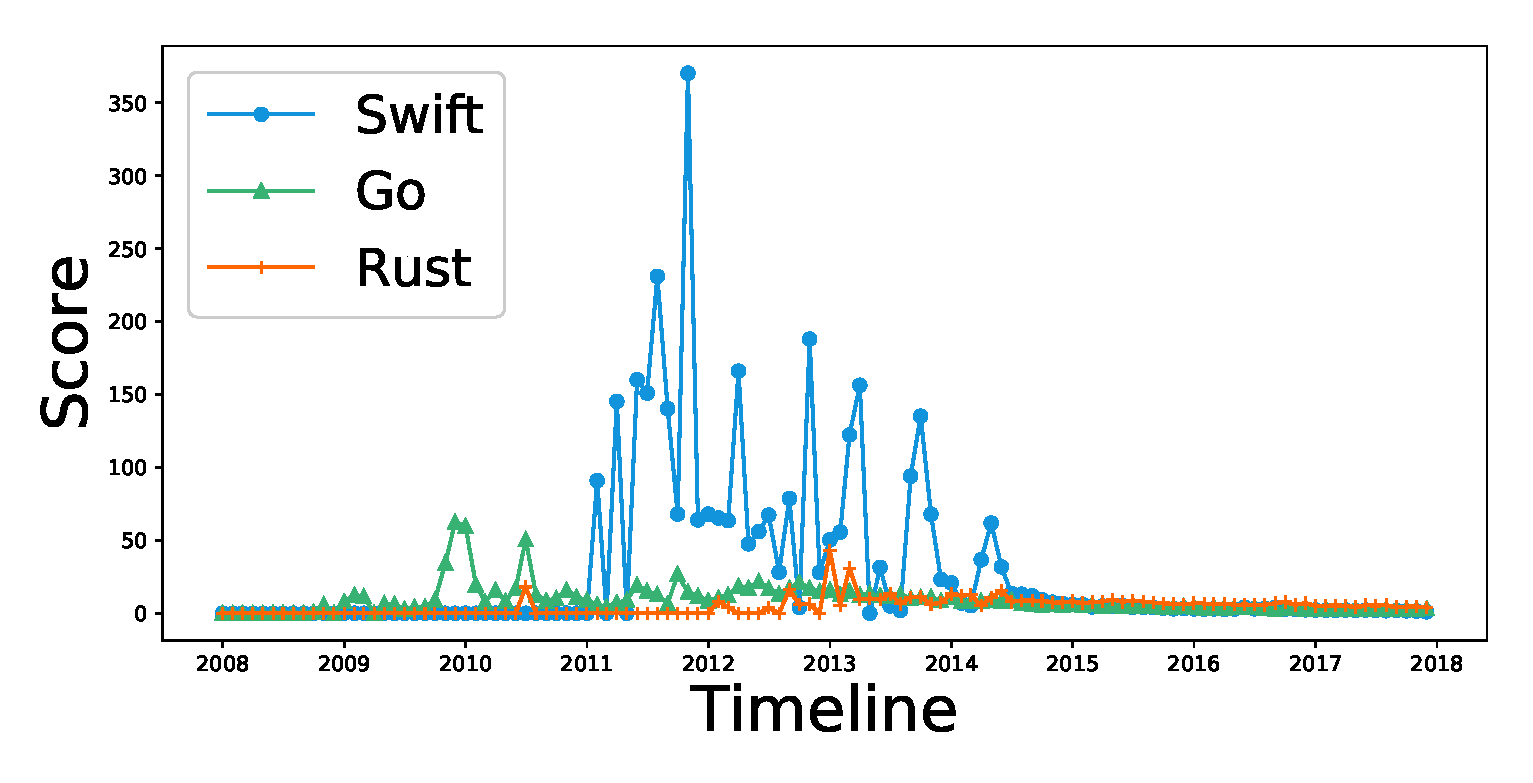
\includegraphics[scale=0.2]{figures/content_quality.eps}
\caption{Post quality of new languages in Stack Overflow}
\label{fig:Content quality}
\end{subfigure}
\begin{subfigure}{0.6\textwidth}
\centering
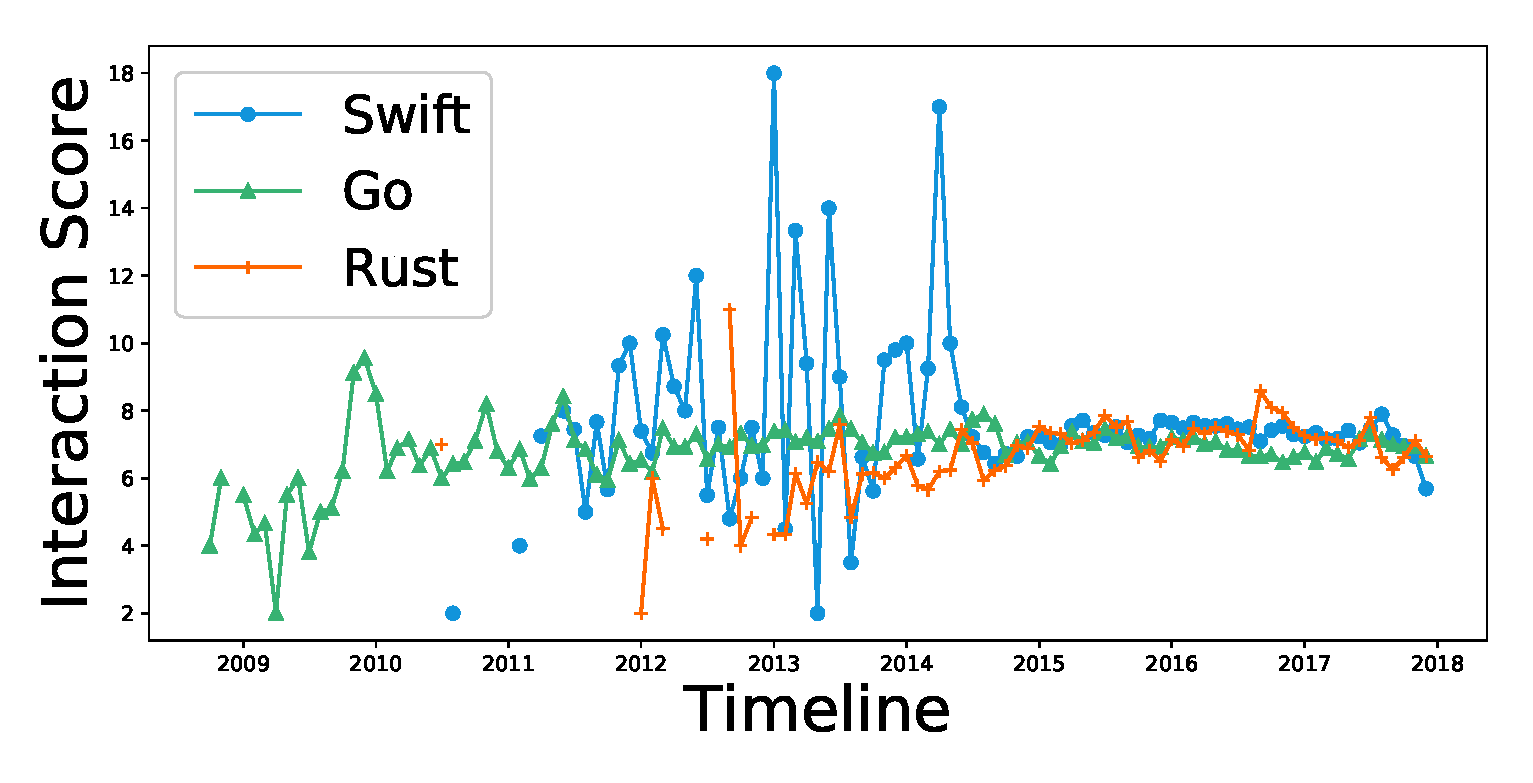
\includegraphics[scale=0.2]{figures/interaction.eps}
\caption{Interaction of developers of new languages with Stack Overflow}
\label{fig:Interaction}
\end{subfigure}
\caption{Post quality of new languages and developers' interaction with new languages vs. time }
\end{figure}

From Figure~\ref{fig:Content quality} it is quite clear that after the release of language, post quality is unstable and the values are very high. The reason behind instability is that the language lacks resources and every new release triggers a set of new questions. The questions of the starting years are less repetitive than the later years\citep{Srba2016}, and it is the reason behind the high value of \emph{score}. Gradually \emph{score} stabilizes into a certain point. In a stable language, users' interaction with Stack Overflow should be minimum and within a range. From Figure~\ref{fig:Interaction}, it is evident that after the first release, \emph{interaction score} also stabilizes to a point which supports our conjecture.

%Continuous up gradation of a feature, documentation  leads a language to its stable point.
To effectively measure the difference of score between consecutive months \emph{first difference} metric \citep{Rasheed2011} has been applied on the score of each language. First difference of score is the difference of score of the consecutive month. \textcolor{green}{The \emph{first difference} technique removes any unobserved variable from data. Moreover, as the data points are taken at a constant interval, the value of the \emph{first difference} works like a differential value.} The first difference is plotted against the release time in Figure~\ref{First difference and release}. In the beginning, the first difference of score was following the release. However, gradually it decreases the level of response which means the language is stabilizing. We can detect a stable point for a language from this point of view. By the stable point, we mean the starting date of the period after the first release of a language when the language is so stable that a single release cannot change or disrupt the development process.

If the first difference of score of a language is within a range, then it has two meanings. First, the language is stable. It does not initiate any significant change in the development lifecycle. Secondly, since most of the Stack Overflow posts are repeated, the contribution of this kind of questions will be omitted in the first difference process. Now, we have the effect of the change of frequency of new questions in the first difference of score. Therefore, the first difference of score within a range means developers are facing fewer problems which are not already answered in Stack Overflow. Hence, we can say we have adequate resources in Stack Overflow on new languages.

\begin{figure}[htbp]
\begin{subfigure}{0.6\textwidth}
\centering
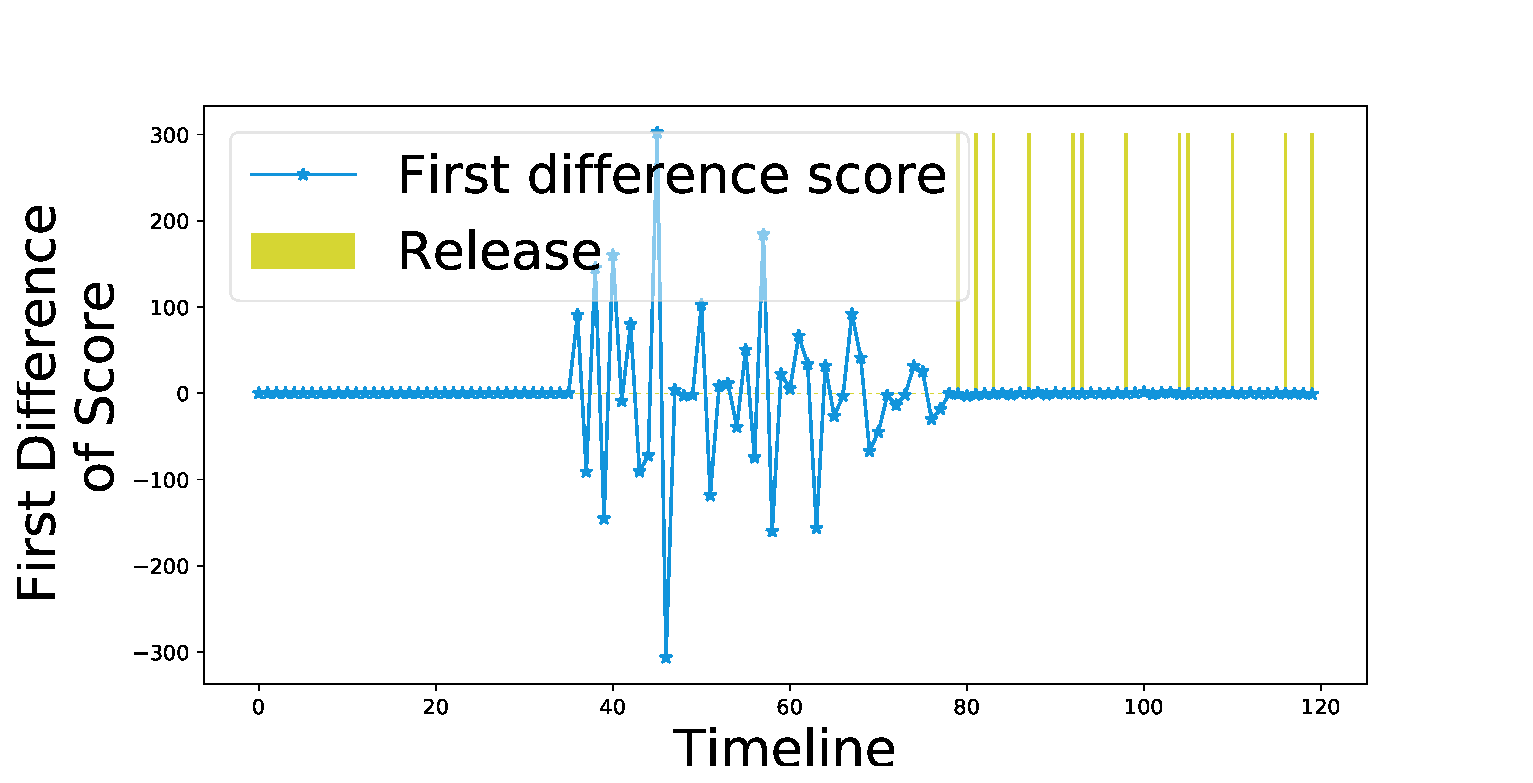
\includegraphics[scale=0.25]{figures/Swift_First_difference_release.eps}
\caption{Swift}
\label{fig:Go_FDR}
\end{subfigure}
\begin{subfigure}{0.6\textwidth}
\centering
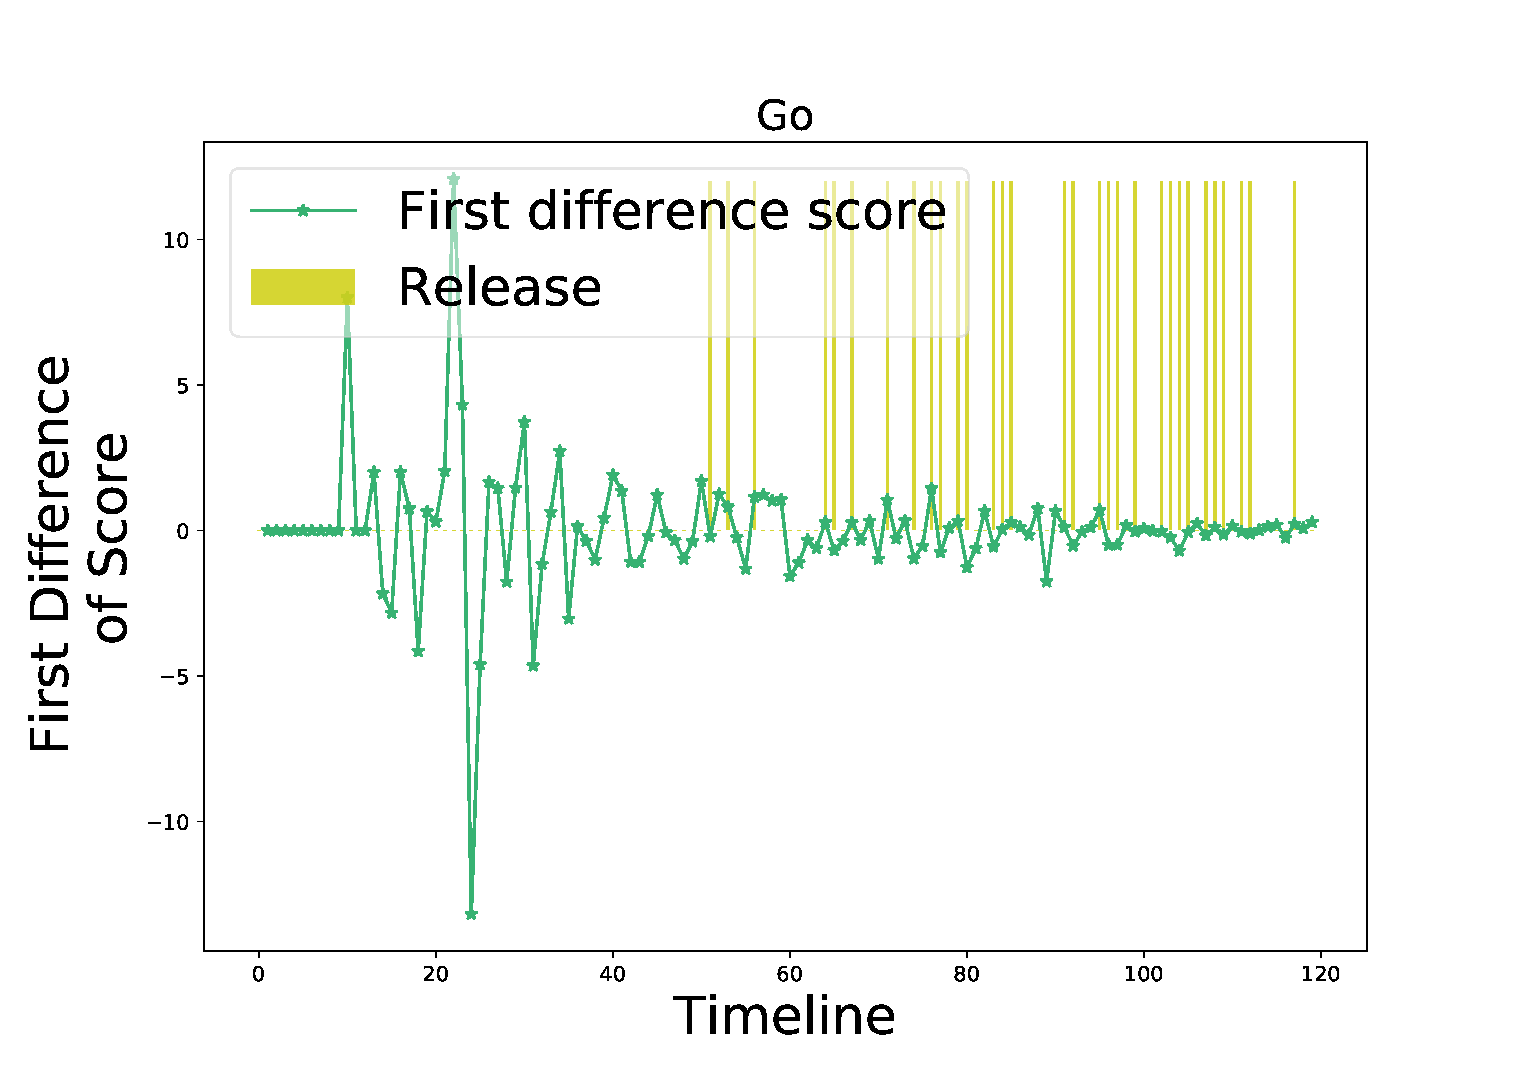
\includegraphics[scale=0.25]{figures/Go_First_difference_release.eps}
\caption{Go}
\label{fig:Swift_FDR}
\end{subfigure}
\begin{subfigure}{0.6\textwidth}
\centering
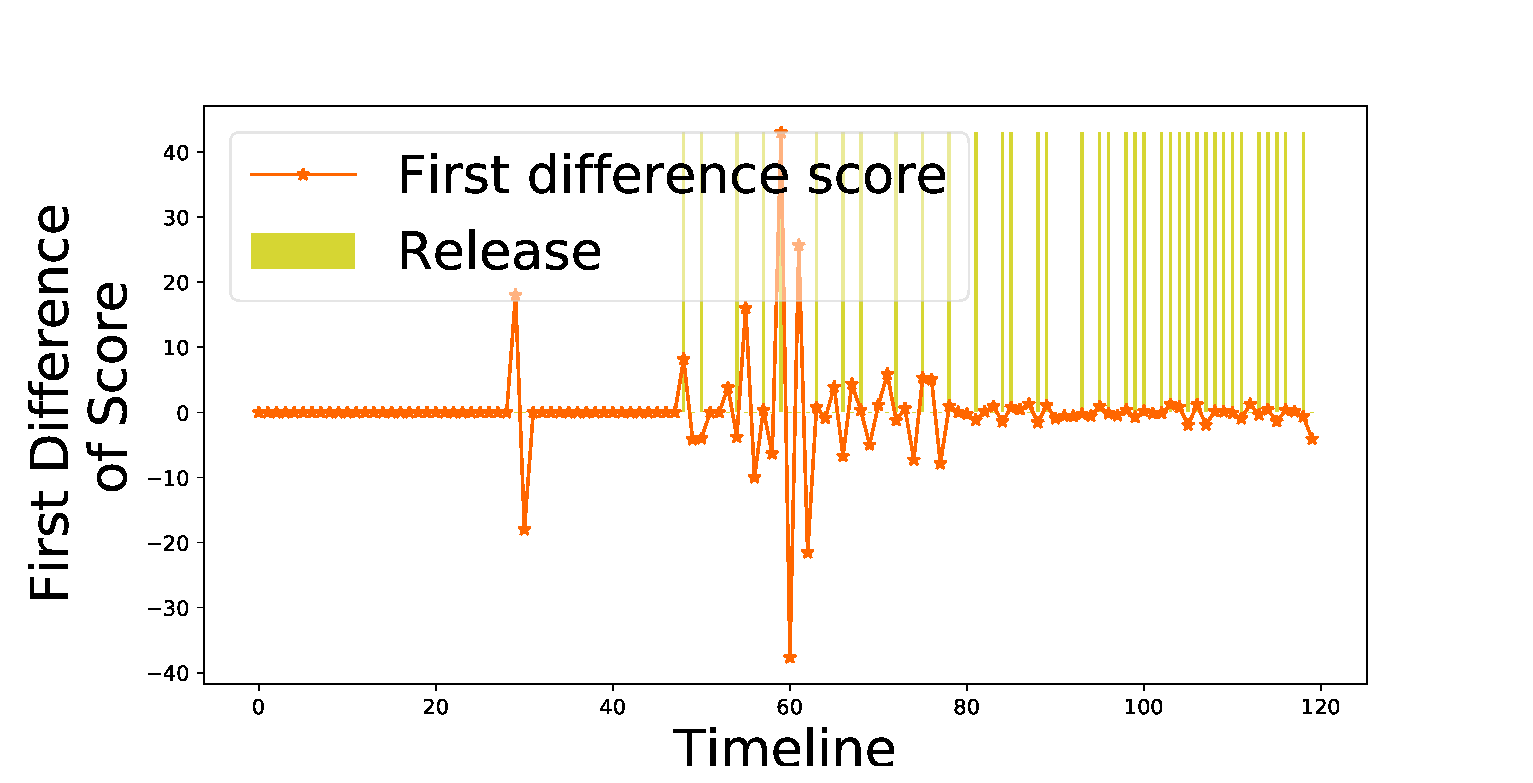
\includegraphics[scale=0.25]{figures/Rust_First_difference_release.eps}
\caption{Rust}
\label{fig:Rust_FDR}
\end{subfigure}
\caption{First difference of the post quality of new languages and release of a new version of new languages.}
\label{First difference and release}
\end{figure}

We defined the stable point as the time point after which value of the first difference is always between -1 and 1. Stable point for each language is presented in Table~\ref{table:Stable point}

\begin{table}[htbp]
\centering
\caption{Stable point of the new languages}
\begin{tabular}{|l|l|l|}
\hline
Language & Release Date & Stable Point Date  \\ \hline
Go & March 1, 2012 & July 1, 2015\\ \hline
Swift & September 9, 2014 & November 1, 2016\\ \hline
Rust & January 1, 2012 & Not reached \\ \hline
\end{tabular}
\label{table:Stable point}
\end{table}

In Stack Overflow the number of Rust developer is too low compared to the other two languages. It is quite common in Stack Overflow that a particular portion of developers leaves or become inactive in  Stack overflow after some time. The post quality of Rust will change quickly after such departure. However, such departure cannot change Go or Swift post quality so frequently as departing developers represent a small percentages of the whole community of these languages in Stack Overflow. That is why our study has found that Rust language has not reached a stable point in Stack Overflow.

\boxtext{\textbf{Finding 2:} In Stack Overflow, we can expect adequate resources of Swift after two years of release while this period is three years for Go. We have found the evidence of having an inadequate resource of Rust language in Stack Overflow.}

\boxtext{\textbf{Finding 3:} The size of an active community can influence the growth of a new language.}

% The significance of stable point is, after the stable point the growth of a language is not affected by a new release. That means quality answers and questions about all the core features are already available in Stack Overflow. We may say a developer will find the answers of all the common questions in Stack Overflow after stable point.ambiguous.
\subsection{RQ3: Relation between the advancement of new languages and its developers' activity}
\label{RQ2}
Being the most used QA site Stack Overflow provides us an insight into the developers' activity pattern. We can get the activity pattern of the developers' of a new programming language from the question-answer frequency of that language. High developers' activity helps to expose special cases and rare bugs of a project. Developers use the issue to inform the language owners about these problems or a particular case. The solution to these problems and bugs led to the growth of the language. Hence, we expect a  relationship between issue and developer's activity pattern. Moreover, developers' activity can also be observed from the number of users, repositories of that language from GitHub. To measure the relationship among variables we have performed the following steps.
\begin{enumerate}
    \item Model Construction (MC)
    \item Model Analysis (MA)
\end{enumerate}
These steps are discussed below.

\textbf{Model construction (MC):} 
We build a regression model to explain the relationship between dependent and explanatory variables. Regression model fits the dependent variable with respect to independent variables. We followed the model construction approach of Harrel et al.\citep{Harrell2015}. While relaxing the linearity assumption, this approach models the nonlinear relationship accurately.
The steps for model construction are described below.
\begin{enumerate}
    \item \emph{Estimation of maximum degrees of freedom:}
    A critical concern in model building is overfitting. Overfitting is most frequent in models that use more degree of freedom than the dataset can support. Hence, we have fixed the maximum degree of freedom for our model. As suggested by Harrel et al.\citep{Harrell2015}  we have fixed  \(\frac{n}{15} \) degree of freedom for our model
    \item \emph{Normality adjustment:}
    We fit our regression models using the Ordinary Least Squares (OLS) technique. OLS assumes the normality in the distribution of the dependent variable. Hence, it is crucial that the distribution of the dependent variable is normal. A widely used approach for conversion into a normal distribution is applying $\ln$ function\citep{pmid25092958}. We have some zero value in our dataset. Therefore in our case, we have used $\ln (x+1) $ to lessen the skew, and better fit the OLS assumption.
    \item \emph{Correlation analysis:}
    Before building the model, we checked the highly correlated explanatory variables. In this step, we have used Spearmen rank correlation as it is resilient to data which is not normally distributed. We have constructed a hierarchical overview of the correlation among explanatory variables. For sub-hierarchies of explanatory variables with correlation $\rho$ \textgreater 0.9, we selected only one element of the sub-hierarchy.
    \item \emph{Fit regression Model:}
    Finally, after selecting explanatory variables and log transformations of dependent variables, we fit our regression models to the data.
\end{enumerate}

\textbf{Model Analysis (MA):} 
We have calculated adjusted $R^2$ to measure the goodness of fit of the model. Adjusted $R^2$ takes into account the bias of additional degree of freedom by penalizing the model for each degree of freedom.
The steps for model analysis are described below.
\begin{enumerate}
    \item \emph{Assessment of Model stability:} 
    Adjusted $R^2$ may overestimate the performance of the model for the curse of overfitting. The performance estimation is taken into account by subtracting the average \emph{optimism}\citep{Efron1986}. The \emph{optimism} is calculated in three steps. First, a bootstrap is created from N samples. Second, a model is fitted on the bootstrap data using the same degree of freedom. Third, \emph{optimism}, the difference between the adjusted $R^2$ of the bootstrap model and the model built in the previous step(original model) is calculated. The process is repeated for 1000 times, and we have got average optimism. Finally, we subtracted the average optimism from original adjusted $R^2$ and got optimism reduced $R^2$.
    \item \emph{Estimation of the power of explanatory variables:}
    To measure the impact of an explanatory variable on a model, we measured the difference in performance between all explanatory variables(full model) and all explanatory variables except one(dropped model). A $\chi^2$ test is applied to the resulting values to detect whether each explanatory variable improves model performance to a statistically significant degree. To estimate the impact, we performed the Wald $\chi^2$ maximum likelihood test. The larger the Wald $\chi^2$ value, the more significant the impact of that particular explanatory variable is\citep{McIntosh2015}.

\end{enumerate}
We can observe the relation between developers' activity pattern and advancement of the language project from two different perspectives: (1) Question count of Stack Overflow and (2) Repository and User count of that language from GitHub. Hence, we performed the process of estimating the relationship for each perspective. We have used open issue count, closed issue count, and the ratio of open issue count with respect to the total number of the issue as the explanatory variable and the question count as the dependent variable to estimate the relationship between issue frequency and developers' activity from  Stack Overflow perspective. According to our methodology, results for the estimation of the relationship between the age and the developers' activity from the \textbf{perspective of Stack Overflow} is presented below.
\begin{table}
\centering

\caption{Coverage model statistics from the perspective of Stack Overflow}
\begin{threeparttable}
\begin{tabular}{|l|l|l|l|}
\hline
       & Swift & Go & Rust \\ \hline
    Adjusted $R^2$   &0.443  & 0.813 &0.924  \\ \hline
    Optimism-reduced $R^2$ & 0.441 &0.802  &0.919 \\ \hline
    Budgeted Degree of freedom & 8 & 8  &8 \\ \hline
%    Degree of freedom spent   & 3 & 4 & 3 \\ \hline
    Open Issue $\chi^2$             & 10 \tnote{*} & 53\tnote{**} & 10\tnote{*}\\ \hline
    Closed Issue $\chi^2$           & 59 \tnote{*}& 251\tnote{**} & 716\tnote{**} \\ \hline
    Ratio of Open Issue $\chi^2$    & 10 \tnote{*} & 63\tnote{**} & 21\tnote{**}\\ \hline
\end{tabular}


\begin{tablenotes}
\item [*] p\textless 0.1 
\item [**] p\textless 0.001
\end{tablenotes}
\end{threeparttable}
\label{table:issue_question relationship}
\end{table}



\begin{enumerate}[wide=0pt, leftmargin=*]
    \item[(MC-1)] \textbf{Estimation of the maximum degree of freedom:} We have 120  points in our dataset. Hence, by Harrel et al.\citep{Harrell2015} we can allow maximum 8 degrees of freedom.
    \item[(MC-2)] \textbf{Normality adjustment:} Question frequency of the new languages is right-skewed. So we have to perform log normality adjustment in this case.
    \item[(MC-3)] \textbf{Correlation analysis:}
    We hierarchically clustered the features by Spearmen $\mid \rho \mid$ value. It is found that the open issue ratio is highly correlated with closed issue count. For the sake of completeness, we have created a model using closed issue count instead of open issue ratio and vice-versa but have not found any change in the performance of the model.
    \item[(MA-1)] \textbf{Assessment of model stability:}
    Table~\ref{table:issue_question relationship} presents the adjusted $R^2$ and optimism corrected $R^2$. From Table~\ref{table:issue_question relationship}, we can say that the model is stable for Swift and Go where the optimism (the difference between Adjusted $R^2$ and Optimism-reduced $R^2$) is 0.002 and 0.005 respectively. However, for Go, the optimism is 0.011. Though the difference is noteworthy, it does not invalidate our model.
    \item[(MA-2)] \textbf{Estimation of the power of explanatory variables:}
    The high $\chi^2$ value of the open issue and the ratio of the open issue to the total number of issue in  Table~\ref{table:issue_question relationship} represents the significant role of these parameters in Stack Overflow. However, they are not that much significant for determining the number of Swift and Rust language questions in Stack Overflow. On the other hand, closed issue ratio is significant for all three languages in determining the number of questions in Stack Overflow which is proved by the high $\chi^2$  value of closed issue in Table~\ref{table:issue_question relationship}. Overall,  the $\chi^2$ value of Swift language is relatively smaller than the other two languages. Hence, we can say that the GitHub issue provides a meaningful and robust amount of explanatory power in describing question frequency of new languages except Swift.
\end{enumerate}
It is quite clear from the adjusted $R^2$ value of Table~\ref{table:issue_question relationship} that there is a relationship between language the growth of a language and the number of questions posted. As seen from Table~\ref{table:issue_question relationship}, the number of closed issues is the most impactful explanatory variable for the Rust language model. Hence, we can say that the number of open issues will significantly influence the number of Rust question in Stack Overflow.
Developers use an issue to ask owners about a new feature and seeking help about any problems. More developers may lead to a high number of issues. Therefore, from GitHub perspective, to model a relationship between issue and the developers' activity we have used User count of that language and Repository count of that language as the explanatory variable and Open issue count as the dependent variable. The relationship between the growth of a language and the developers' activity from the perspective of GitHub is presented below.
\begin{table}
\centering
\caption{Coverage model statistics for relationship from the perspective of GitHub}
\begin{threeparttable}
\begin{tabular}{|l|l|l|l|}
\hline
       & Swift & Go & Rust \\ \hline
    Adjusted $R^2$   &0.755  & 0.907 &0.862 \\ \hline
    Optimism-reduced $R^2$ & 0.751 &0.905  &0.859 \\ \hline
    Budgeted Degree of freedom & 8 & 8  &8 \\ \hline
%    Degree of freedom spent   & 4 & 4 & 3 \\ \hline
    User $\chi^2$             & 64 \tnote{*} & 215\tnote{*} & 50\tnote{*}\\ \hline
    Repository $\chi^2$           & 289 \tnote{**}& 19\tnote{**} & 192\tnote{**} \\ \hline
\end{tabular}
\begin{tablenotes}
\item [*] p\textless 0.1 
\item [**] p\textless 0.001
\end{tablenotes}


\end{threeparttable}
\label{table:github_question relationship}
\end{table}



\begin{enumerate}[wide=0pt, leftmargin=*]
    \item[(MC-1)] \textbf{Estimation of the maximum degree of freedom:}  To answer this question we have used the same dataset used in the previous step. Hence, we can allow a maximum of 8 degrees of freedom.
    \item[(MC-2)] \textbf{Normality adjustment:} Like the previous step, we have applied a log transform to normalize the dependent variable(open issue count).
    \item[(MC-3)] \textbf{Correlation analysis:}
    We have used two feature to build this model. Hence, instead of hierarchical clustering, we just calculated the Spearmen $\mid \rho \mid$ value between \emph{user count} and \emph{repository count}. It is found that they are not correlated.
    \item[(MA-1)] \textbf{Assessment of model stability:}
    Table~\ref{table:github_question relationship} presents the adjusted $R^2$ and optimism reduced $R^2$. From Table~\ref{table:github_question relationship} the optimism for each language is \textless 0.01 which ensures the stability of the model.
    \item[(MA-2)] \textbf{Estimation of the power of explanatory variables:}
    The issue is associated with the developers' experience. Hence, we expect `User' parameter to be an important feature in determining the number of open issue in the official GitHub repository of new languages. Table~\ref{table:github_question relationship} shows a high $\chi^2$ value of user count parameter, which supports our conjecture about the significance of the number of users in determining the number of open issue in GitHub. We have also found that Rust has relatively less user in GitHub compared to the other two languages which are expressed in the $\chi^2$ value of `User' parameter for Rust. The high $\chi^2$ value of the repository parameter for Swift and Rust language represents the significance of the number of the repository in determining the number of Swift and Rust open issue. However, the number of repositories is less significant in determining the number of open issue in the Go GitHub repository compared to the other two languages.
\end{enumerate}
From the adjusted $R^2$ value of Table~\ref{table:github_question relationship}, it is clear that there is a strong relationship between developers' GitHub activity and the number of open issue in the official repository of that respective language. 

\boxtext{\textbf{Finding 4:} There is a relationship between developers' activity pattern and growth of the language.}

\boxtext{\textbf{Finding 5:} The number of open issues of Rust in GitHub significantly influenced the number of question on Rust in Stack Overflow.}

\boxtext{\textbf{Finding 6:} The open issue count of Swift and Rust is highly dependent on the number of repositories of that language in GitHub.}


Every new release impacts the growth of a programming language. The developers' activity after a new release can give us an idea about the relationship between developers' activity pattern and the growth of a language. To observe the developers' activity pattern after a new release, we have collected all release dates of new languages from GitHub and then plotted them alongside question, issue, and repository count.

\begin{figure}[h]
 \centering
\begin{subfigure}{0.6\textwidth}
\hspace{40pt}
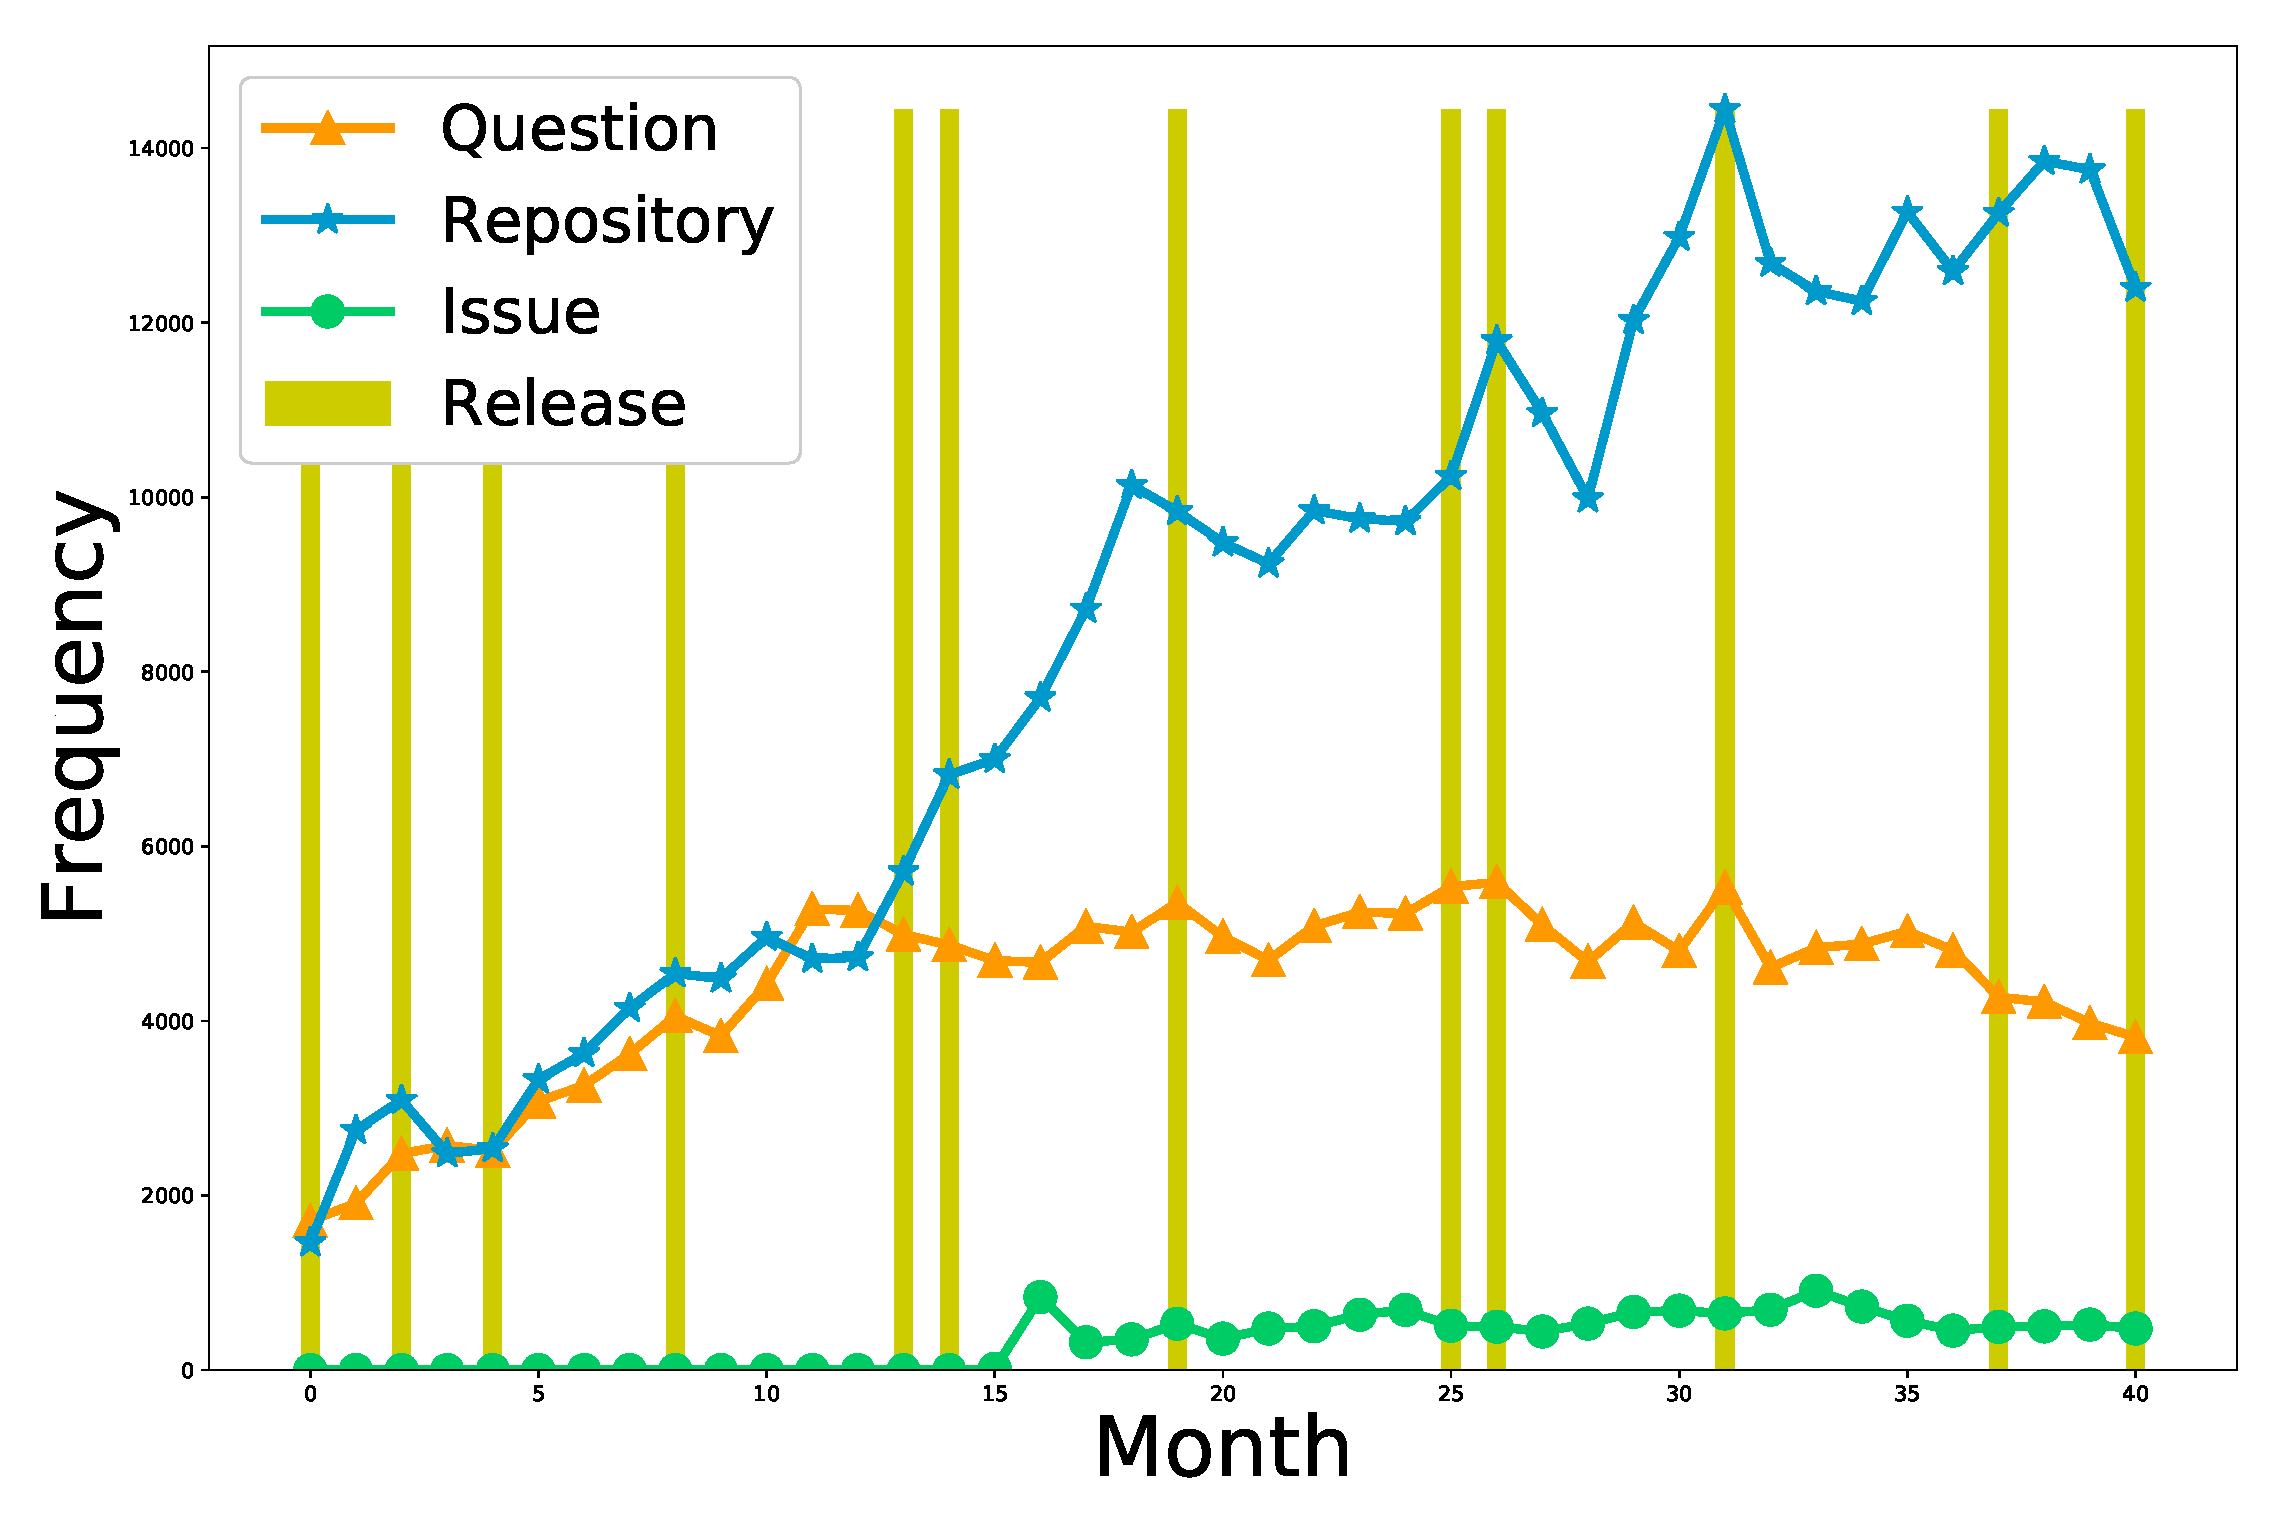
\includegraphics[scale=0.14]{figures/Swift_release_and_user_behaviour} 
\caption{Swift language}
\label{fig:Question count for Swift}
\end{subfigure}
\begin{subfigure}{0.6\textwidth}
\hspace{40pt}
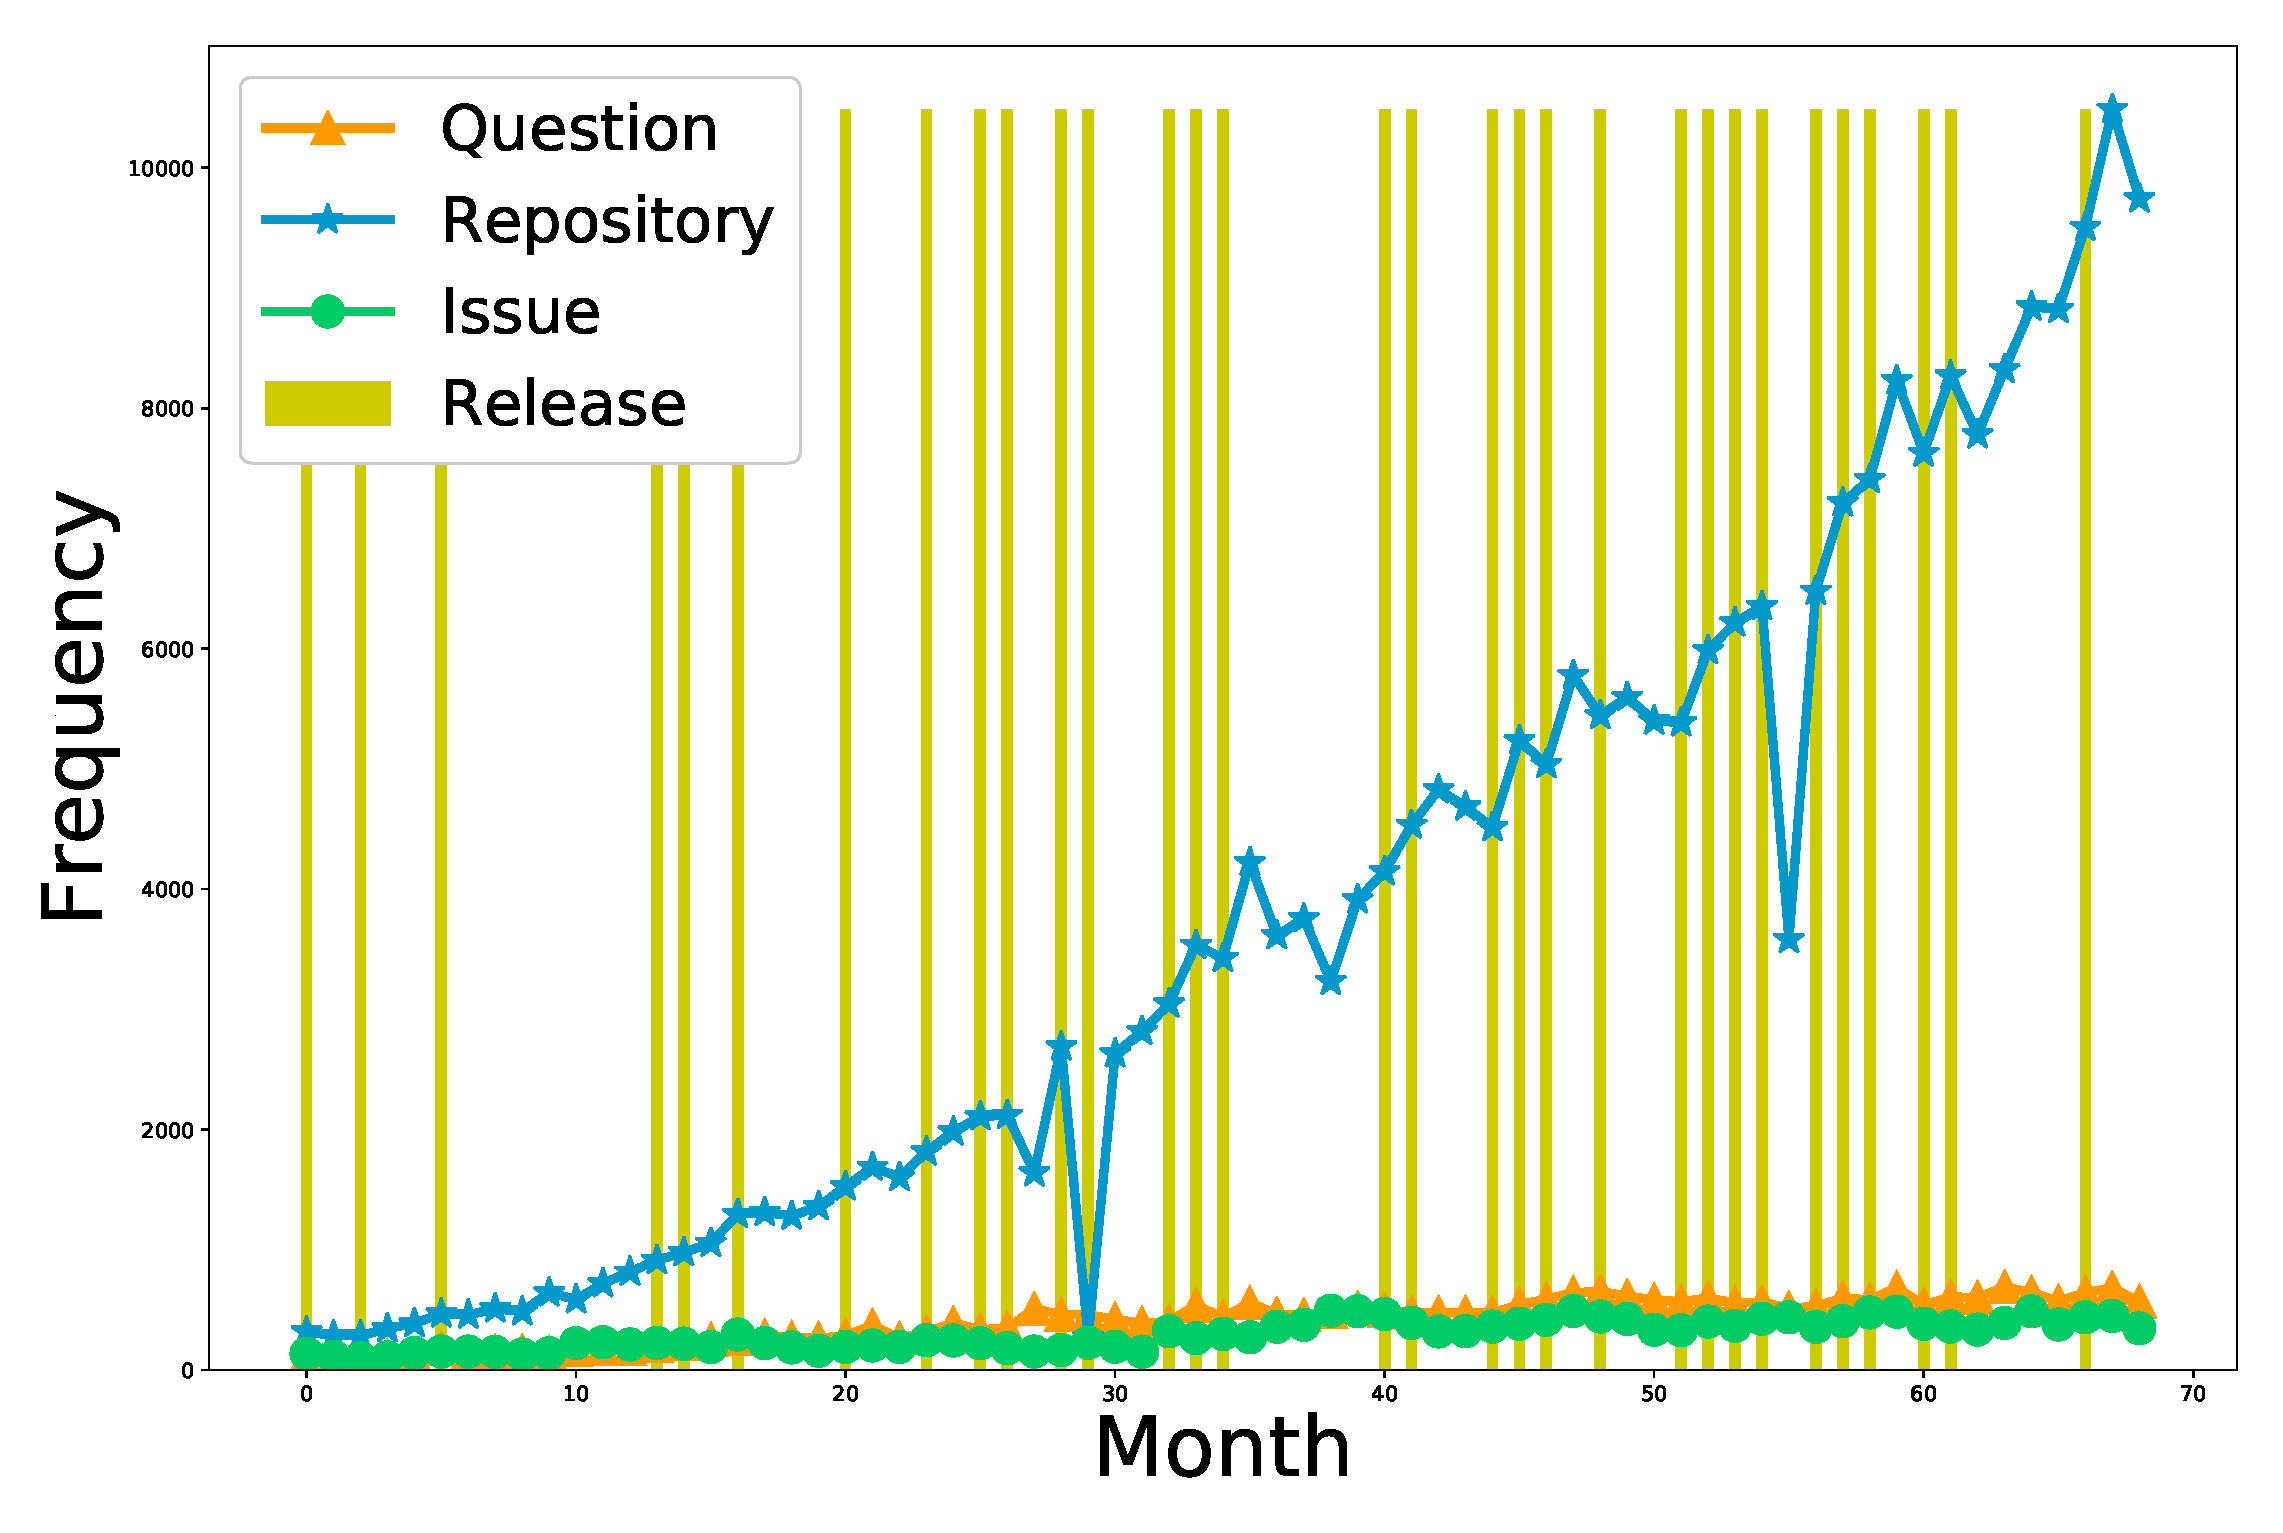
\includegraphics[scale=0.14]{figures/Go_release_and_user_behaviour}
\caption{Go language}
\label{fig:Question count for Go}
\end{subfigure}
\begin{subfigure}{0.6\textwidth}
\hspace{40pt}
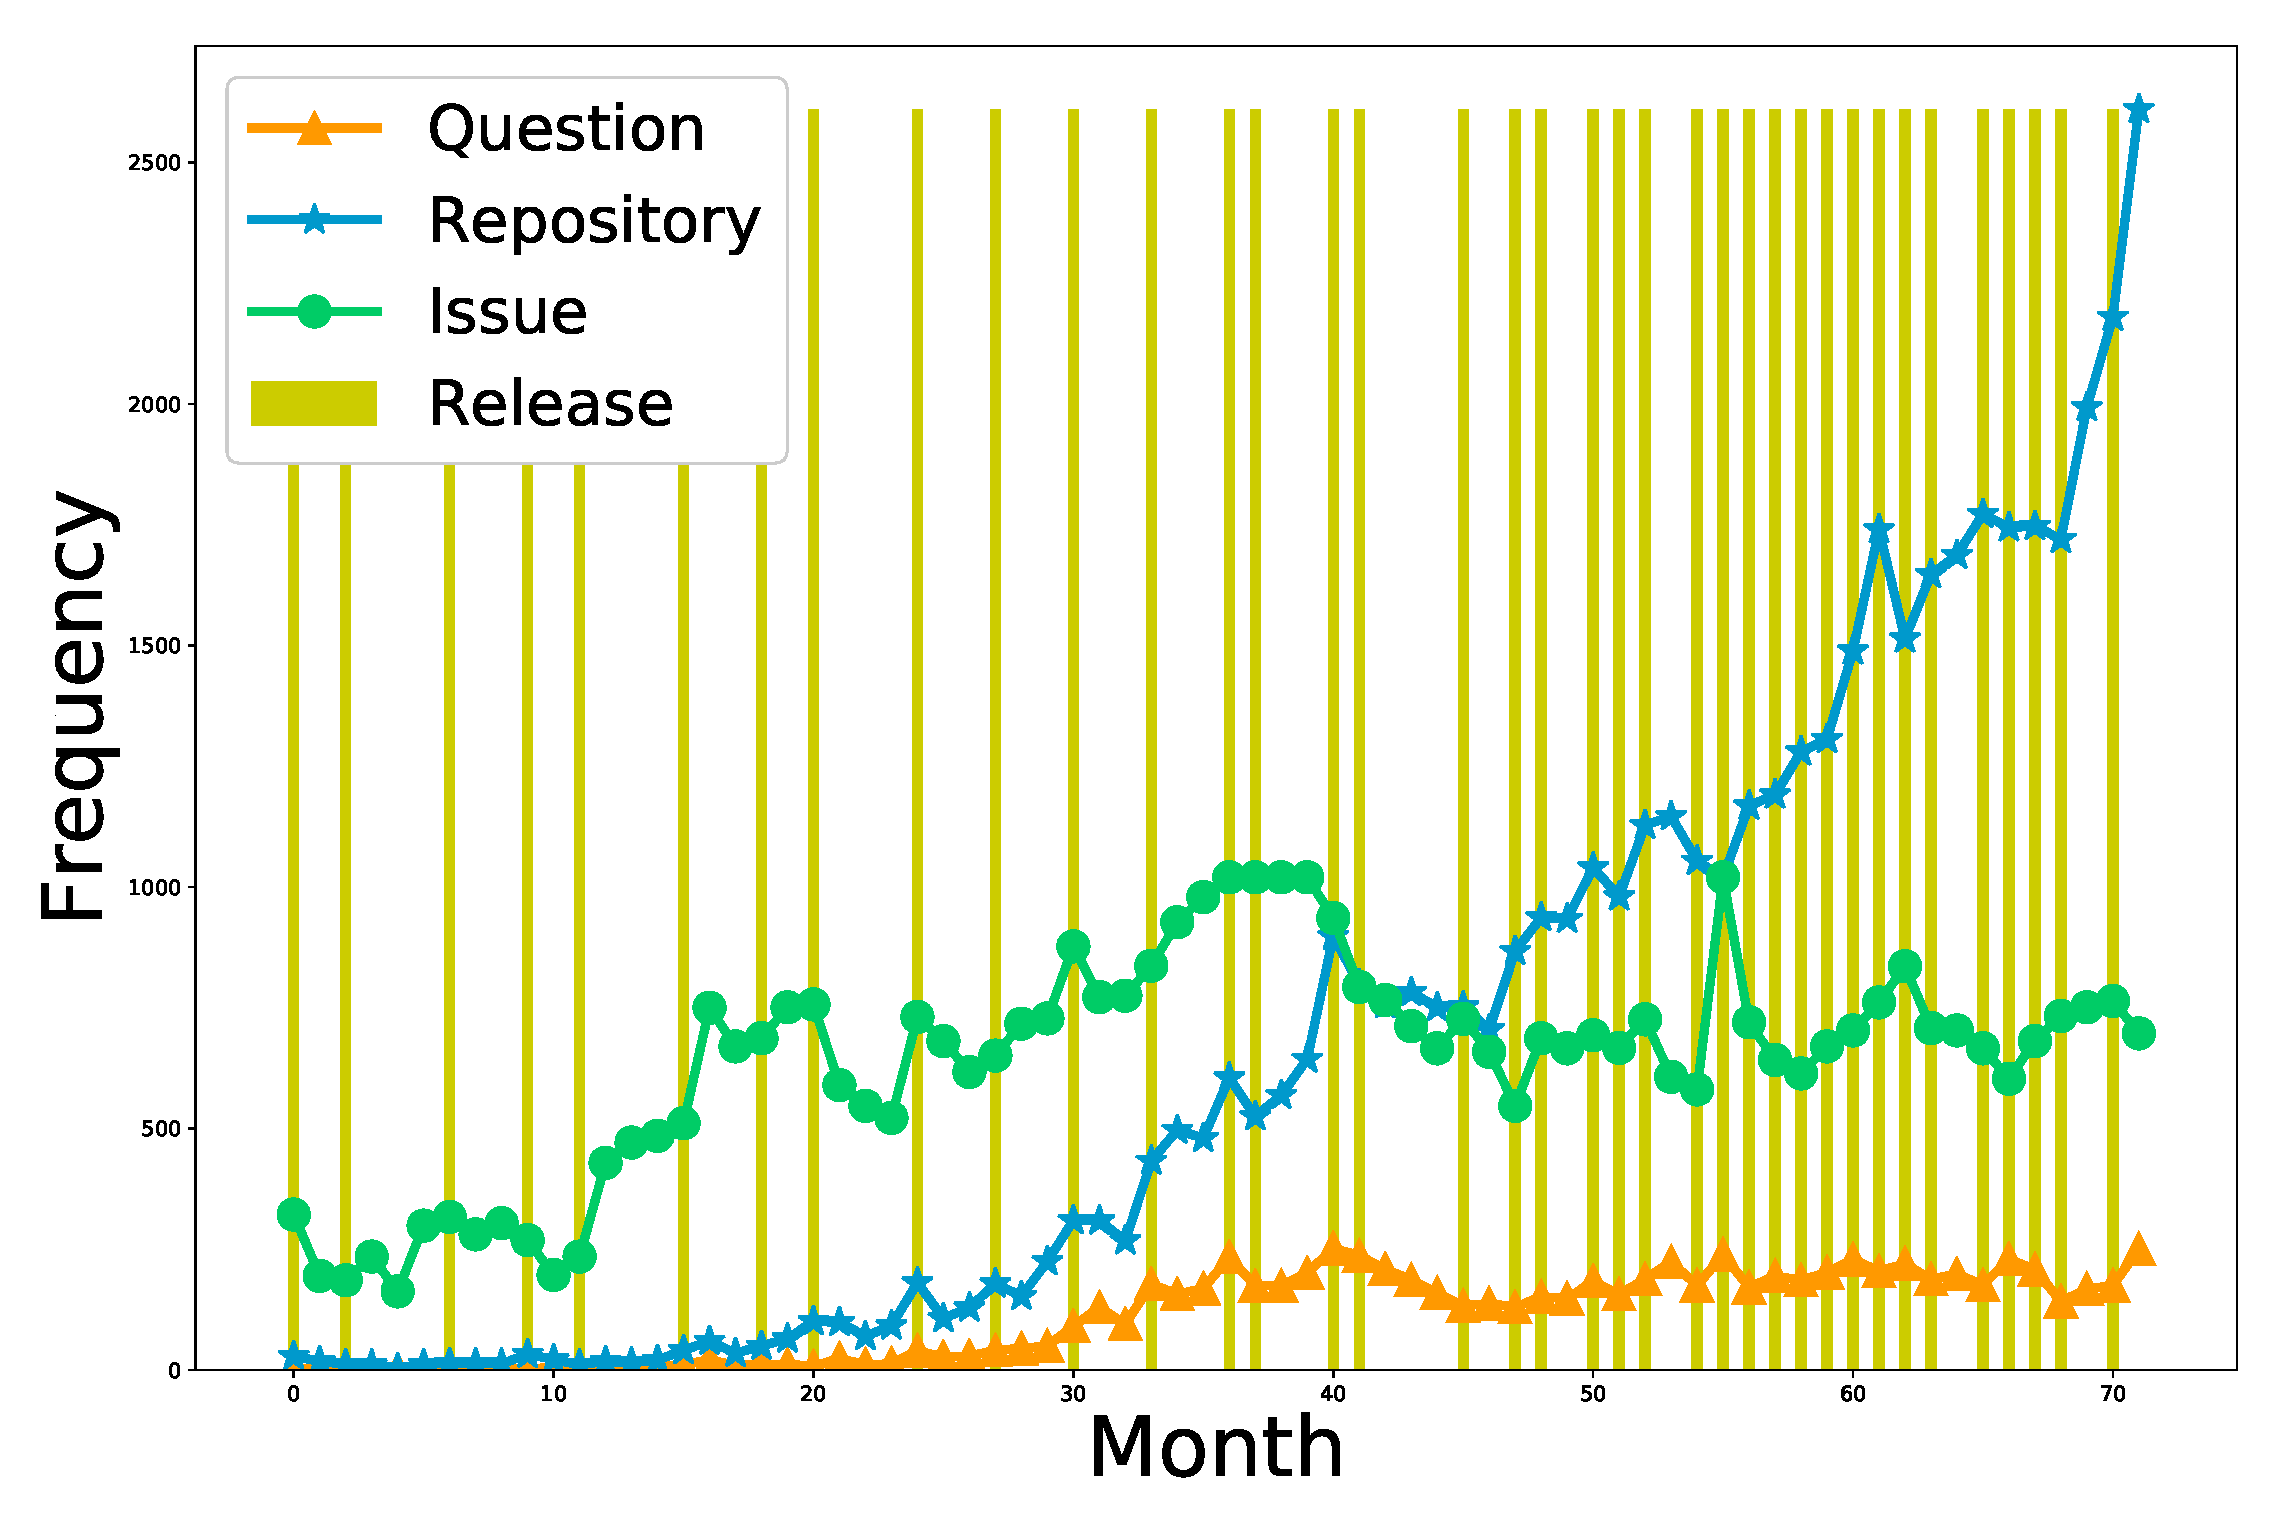
\includegraphics[scale=0.14]{figures/Rust_release_and_user_behaviour}
\caption{Rust language}
\label{fig:Question count for Rust}
\end{subfigure}
\caption{Release of a new version and activity pattern of the developers of respective languages}
\label{fig:Release and user behavior}
\end{figure}
Each sub-figure shows the response after the release of a new version. That means developers' activity is influenced by the benefits, features, and bugs of the new release. This trend is also visible  in question count i.e., question count increases after each release (Figure~\ref{fig:Release and user behavior}). However, we observed that issue count of Swift is less influenced than that of the other two languages. For tracking bugs and language problem,  Go\footnote{https://Golang.org/project/} and Rust\footnote{https://github.com/Rust-lang/Rust/blob/master/CONTRIBUTING.md} use only GitHub issue tracker. On the other hands, besides using GitHub issue tracker, Swift\footnote{https://Swift.org/contributing/\#reporting-bugs} uses their own JIRA\citep{wiki:JIRA} instance for tracking bug\footnote{https://bugreport.apple.com/}. This is a likely cause of the difference, and as a result, the issue count of Swift represents a portion of the actual issue(bugs), and so it is less influenced by a new release than the other two languages. We have tested this hypothesis using statistical testing. We have performed Wilcoxon signed-rank test between the question, repository and issue count of the month before release and the count of the month of release. The result is presented in Table~\ref{table:release_impact}. However, only the change in repository count was significant. The reason behind significance is after each new release developers create a new repository to test the new features without altering the production version of the software. Hence, the number of repository increases after a new release. Though we can observe that the question and issue count 
\begin{table}
\centering
\caption{Wilcoxon signed rank test result for the comparison of change between before and after of a release.}
\begin{tabular}{|c|c|c|c|}
\hline
\multicolumn{1}{|l|}{Language} & \begin{tabular}[c]{@{}c@{}}Question\\ p value\end{tabular} & \begin{tabular}[c]{@{}c@{}}Repository\\ p value\end{tabular} & \begin{tabular}[c]{@{}c@{}}Issue\\ p value\end{tabular} \\ \hline
Swift                          & 0.583                                                      & \textless{}0.01                                              & 0.6                                                     \\ \hline
Go                             & 0.149                                                      & \textless{}0.01                                              & 0.433                                                   \\ \hline
Rust                           & 0.473                                                      & \textless{}0.01                                              & 0.2                                                     \\ \hline
\end{tabular}
\label{table:release_impact}
\end{table} are responding with the release of a new version, it is statistically insignificant according to the Wilcoxon signed-rank test. To find the reason behind this insignificance, we conducted a further investigation. We noticed that the spikes in question and issue count curve does not appear immediately after a release. Rather, it appears after a variable time gap. Thus, the change in question and issue count is statistically insignificant.



\subsection{RQ5: Characteristics of answer pattern of new languages}
\label{RQ4}
In Stack Overflow, the community size and age of a language are most likely to influence the answer interval. With time, the answer interval is likely to be decreased. To observe the anticipated change in intervals of new languages, we extracted several features from Stack Overflow like frequency of questions, questions without having any answer (no answer), questions having an accepted answer (accepted answer) and questions without an accepted answer (no accepted answer). An insight into the evolution of new languages, one top-tier language (Java) and mid-category language (Python)
are presented in Figure~\ref{fig:Evolution of new languages}. It is clear from Figure~\ref{fig:Evolution of new languages} that the evolution pattern of Python is quite similar to Swift, while Java shows a different pattern compared to all three new languages. A natural deduction is  that Java was released long before and was already a mature language prior to the inception of SO.  Hence, the community interaction at the initial period of Java is missing in our dataset. On the other hand, although Python was also released long before the inception of SO, its  use increased significantly after 2010\citep{TIOBE:index}.

\begin{figure}[htbp]

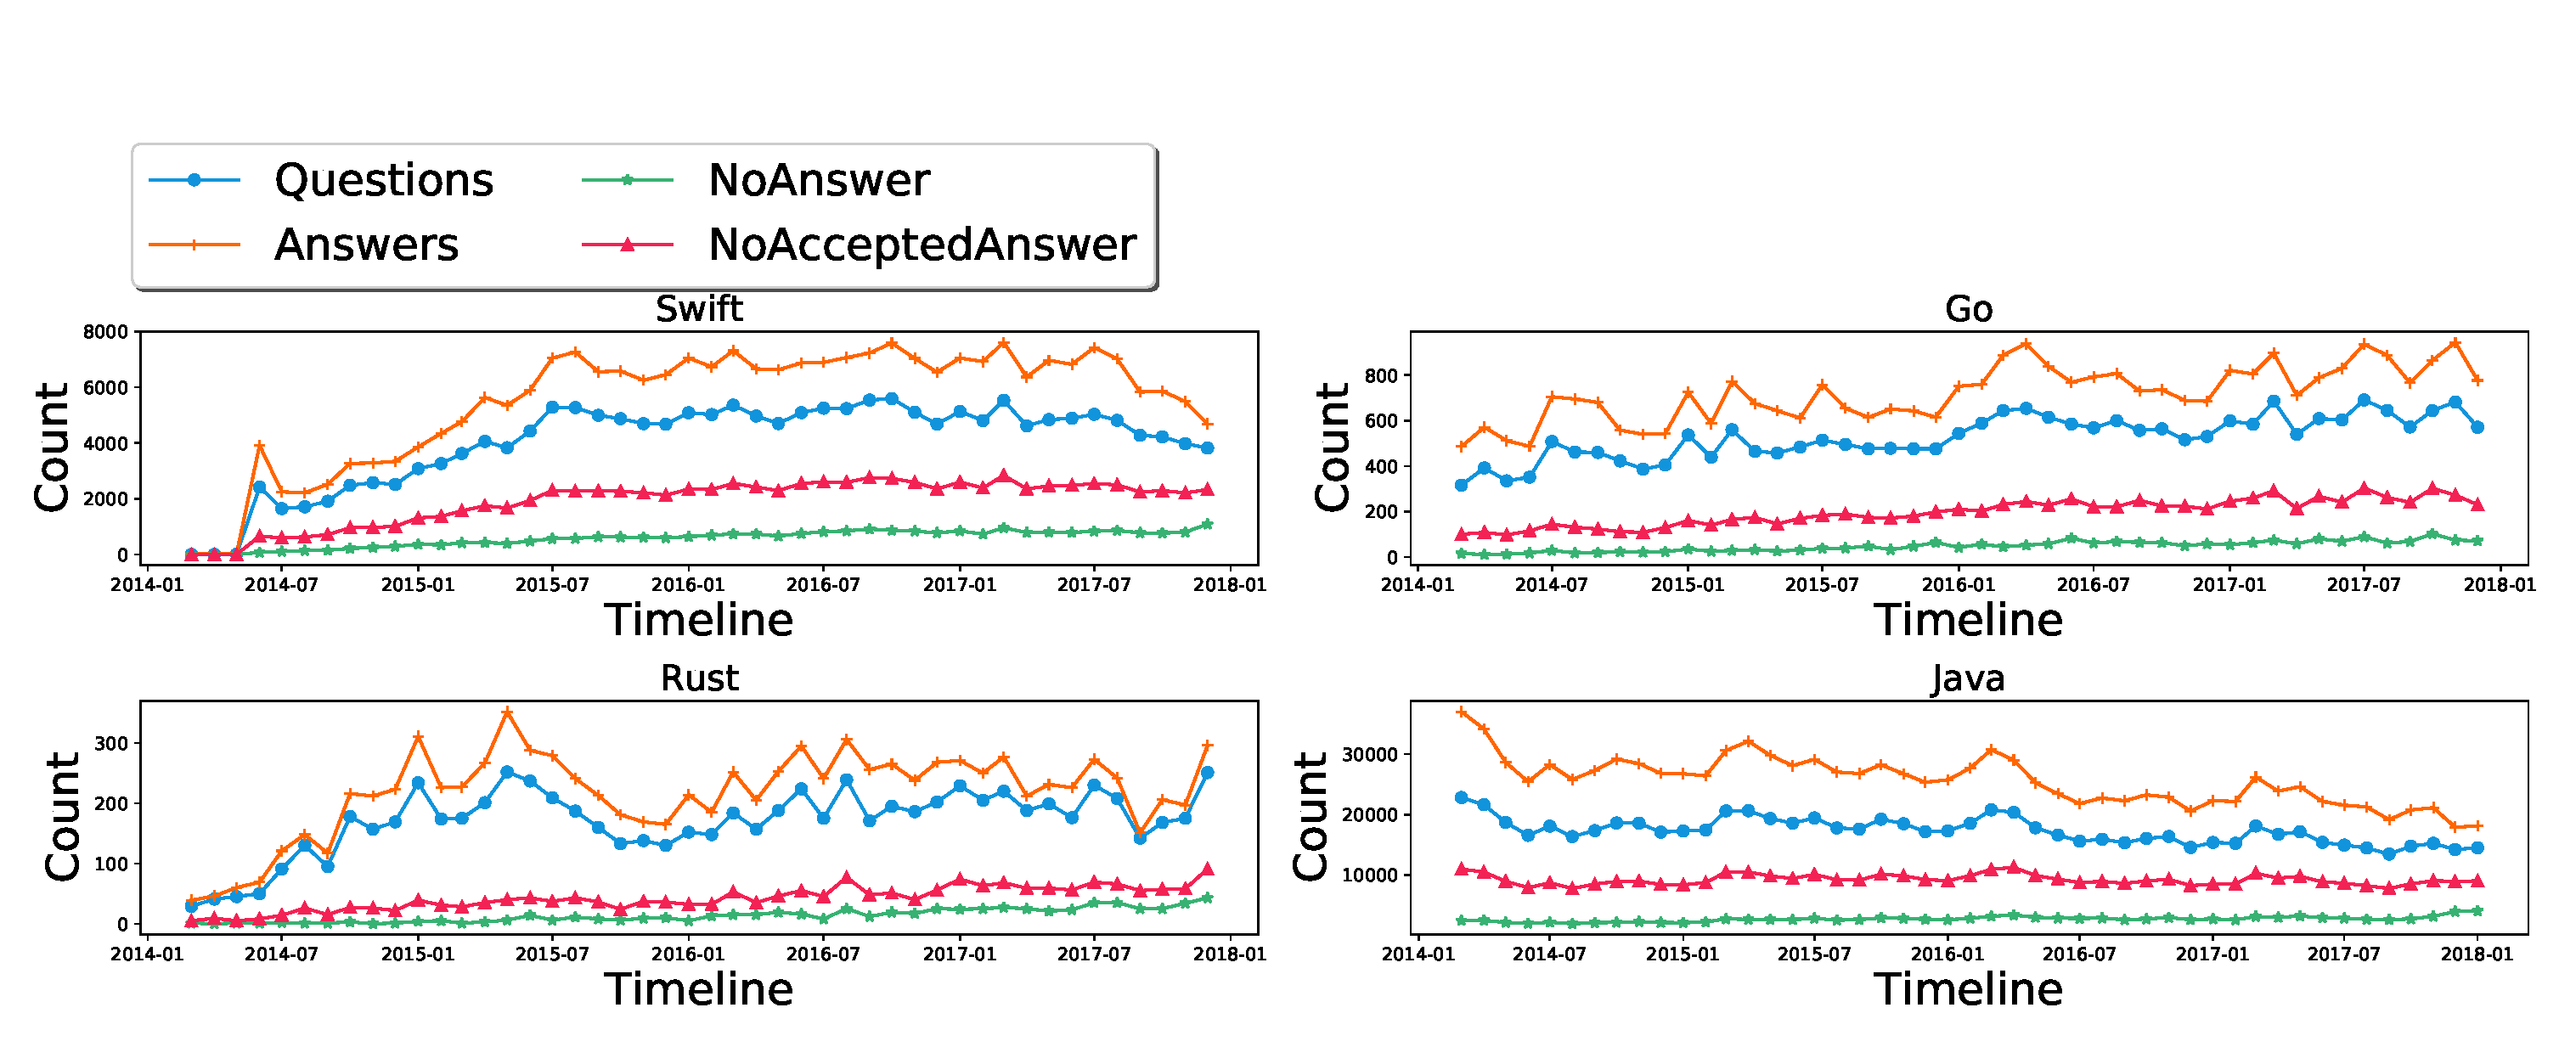
\includegraphics[scale=0.28]{figures/Evolution.eps} 
\caption{Question, No answer, Accepted answer, and No accepted answer count of languages in Stack Overflow}
\label{fig:Evolution of new languages}
\end{figure}

\iffalse
It is prominent in Figure~\ref{fig:Evolution of new languages} that the question count curve of Swift language (Figure~\ref{fig:Attributes of Swift Language}) is much smoother than the other two languages. The reason of smoothness is related to the closed issue ratio. Earlier, we have described the two states of GitHub issue. Based on the two states, we defined the closed issue ratio as,

\begin{equation}
{Closed \quad issue \quad ratio=}
\left[\dfrac{Closed\quad issue}
{Closed\quad issue+Open\quad issue}\right]
\label{eq:Closed Issue Ratio}
\end{equation}

We can say that the closed issue ratio means how much problems have been solved. It can be used as a measure of an active development team. Closed issue ratio one means all problems that were raised in that month were solved. We collected all the issue of the official repositories of new languages and calculated closed issue ratio,

\begin{table}[]
%\centering

\begin{tabular}{|l|l|l|l|}
\hline
 Language& Mean& Variance& Median\\ \hline
 Swift &  0.984  & 0.001 & 0.993 \\ \hline
 Go    &  0.901  & 0.01  & 0.917 \\ \hline
 Rust  &  0.95   & 0.006 & 0.984 \\ \hline

\end{tabular}%

\caption{Statistics of the closed issue ratio of new  languages.}
\label{table:Issue ratio}
\end{table}
From Table~\ref{table:Issue ratio}, we can say Swift has a very active development team with the closed issue ratio close to one. Maybe that is why the question frequency for Swift is smoother than the other two languages.
\fi

Based on the stable date point of new languages presented, we have defined two states for languages (1) Evolving state: the language has just been released, it lacks experts and other resources in Stack Overflow, and (2) Matured State: the language has a stable release with a support community. The details of the stable date point is presented in  in section \ref{RQ1}. Table~\ref{table:States of languages} presents the duration of these states for new languages.
\begin{table}
%\resizebox{\textwidth}{!}{%
\caption{Duration of the evolving and matured state of new languages}
\begin{tabular}{|l|l|l|}
\hline
 Language & Evolving State& Matured State \\ \hline
% Swift & 01/09/14-30/04/16 & 01/05/16-31/12/17  \\ \hline
 Swift & September 2014-October 2016 & November 2016-December 2017  \\ \hline
 Rust & N/A & N/A \\ \hline
 Go & March 2012-June 2015 & July 2015-December 2017 \\ \hline
\end{tabular}%
%}
\label{table:States of languages}
\end{table}
Every answer and question of Stack Overflow is associated with a ``Creation-Date". For each question, we collected all the answers of these questions and by using the ``Creation-Date", we have measured the interval between question and the first answer.
\textcolor{green}{ We must know the distribution  of our data before testing the hypothesis. From the Shapiro-Wilk test\citep{SHAPIRO1965} we found that the distribution of first answer interval distribution does not follow normal distribution. Since non-parametric tests do not assume any distribution, it is widely used in cases where the data does not follow the normal distribution\citep{Mann1947}}. We performed the Mann-Whitney U test which is a non-parametric test to establish the conjecture that it takes more time in the \emph{evolving state} than the \emph{matured state} of their age to have the first answer. The result is presented in Table~\ref{table:Mann-Whitney Test answer interval between states}.


\begin{table}
\centering
\caption{Mann-Whitney U Test result for comparison of the first answer interval between matured and evolving state of new languages}
\begin{tabular}{|l|l|}
\hline
 Language & p value \\ \hline
 Swift & \textless 0.01  \\ \hline
 Rust & Not found \\ \hline
 Go &   \textless 0.01 \\ \hline
\end{tabular}%
\label{table:Mann-Whitney Test answer interval between states}
\end{table}

From the Mann-Whitney test result presented in Table~\ref{table:Mann-Whitney Test answer interval between states}, we have found that only the Swift and Go languages reject the null hypothesis which means that the difference is significant for Swift and Go languages.\\
% According to the release date, Swift is the youngest of these three languages. As a result, when the age is equally divided, it received a small period as evolving state. Even, it may not have reached the matured state yet. On another note, Swift is the direct descendent of Objective-C, and it inherits many libraries and community support from Objective-C. Hence, it may not have an evolving state and started its evolution direct from the matured state. Either of these can be the reason behind the null hypothesis support for Swift.
There may be some differences between topics discussed in the evolving state and the matured state. To test the conjecture, we divided the questions of each language into two states and extracted 10 topics from each state. But the difference was not noticed between the topics. That is because while we are selecting a few topics from large set sub-topics grouped into common programming language topics. To overcome the problem, we extracted 50 topics from each state of each language with their percentage in that stage. If a topic does not appear at both stages, or if their percentage difference is greater than or equal to 2, then we considered that the topic belongs to that stage in which it is most commonly seen. We have tested with various threshold and selected two because otherwise, some topics which are common to all languages irrespective of the stage may appear. Now using this criterion we can identify the topic shift between states of languages.
\begin{enumerate}
\item \textbf{Topics of Swift Language in Evolving State:} During the evolving period, Swift developers mostly talked about language integration and equivalence. Since, in this period, the transition from Objective-C to Swift has just happened, developers were trying to transfer their codebase from Objective-C to Swift. Other popular topics in this state are the use of \emph{alamofire} (a HTTP library) and audio, video controller API of Swift.
\item \textbf{Topics of Swift Language in Matured State:} During the matured state, Swift developers are  mostly concerned about advanced features like ORM, advanced view controllers (segue), and threading. One thing prominent from the data that in matured state Swift developers are asking more questions related to game development such as different type of kits to handle 2D and 3D graphics (sprite kit, scene kit, etc.). The change might be associated with the availability of high-end phones in recent years.\citep{Aleem2016,Gavalas2011}
\item \textbf{Topics of Go Language in Evolving State:} During the evolving state, Go developers discussed compiling issues, compiler path, data types, and type conversion. It seems that developers are trying to understand the syntax and usage of that language. Another common topic in this stage using simple HTTP, TCP, and socket server and encryption technology. As Go is mostly used in the server-side, developers are trying to identify Go's potential by deploying sample project or mimicing old project in the new language.

\item \textbf{Topics of Go Language in Matured State:} In the matured state, Go developers were concerned about HTTP web servers like Gin and  Martini, advanced features like ORM (GORM, GRAIL), and container deployment system Docker, Kubernetes. It is clear that developers are mostly concerned about delivering and deployment system  in this stage.
\end{enumerate}

With the process of evolution, it is expected that the number of unanswered questions will be decreased. To verify this conjecture, we have calculated the unanswered-question ratio for each month. By unanswered question ratio, we mean the ratio of the questions without any answer. We have defined the unanswered question ratio as,

Unanswered question ratio $ = \dfrac{\sum \text{Unanswered questions}}{\sum \text{Questions}}$
\iffalse
\begin{equation}
{\splitdfrac{\quad  \quad Unanswered}{question \quad ratio=}}
\left[\dfrac{\sum Unanswered \quad questions}
{\sum Questions}\right]
\label{eq:Unanswered Question Ratio}
\end{equation}
\fi

The Unanswered question ratio against time is presented in Figure~\ref{fig:Unanswered-question ratio}.
\begin{figure}[htbp]
\centering
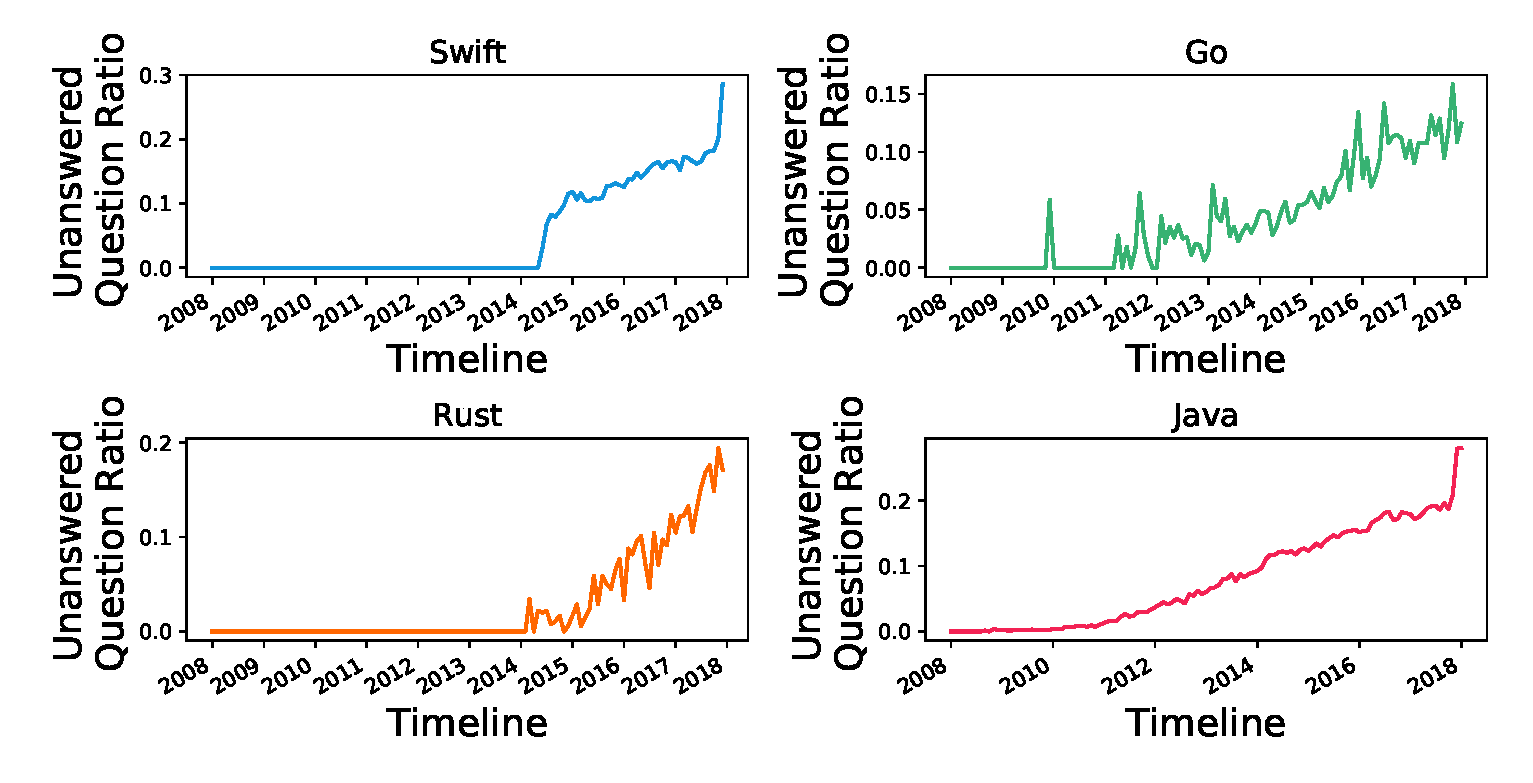
\includegraphics[scale=0.38]{figures/UnansweredQuestionRatio.eps}
\caption{Unanswered-question ratio in Stack Overflow}
\label{fig:Unanswered-question ratio}
\end{figure}


Figure~\ref{fig:Unanswered-question ratio} represents the contrariwise scenery of our assumption. As the day goes by, the unanswered question ratio increases. In one sense, we can say that the answer pattern for new languages and matured languages are the same as in both cases the unanswered question ration increases. However, we can observe two interesting phenomena from these results. First, the change ratio is smoother for matured language while it is notched for new languages except Swift. The reason for the jagged curve may be the absence of active expert developers. Inactive expert developers can change the ratio of the unanswered question by being active for a short time. That is why the curve for Go and Rust are jagged. Being the direct successor of Objective-C, Swift language has avoided this phenomenon. Second, Swift language starts its rise from a certain level which is caused by topic and question inheritance from Objective-C.

To compare growth, we plot the median time to get the first answer and the accepted answer of new languages, one top-tier language (in this case Java), and mid-category language (Python).
\begin{figure}[htbp]
\begin{subfigure}{0.6\textwidth}
\centering
\hspace{-3cm}
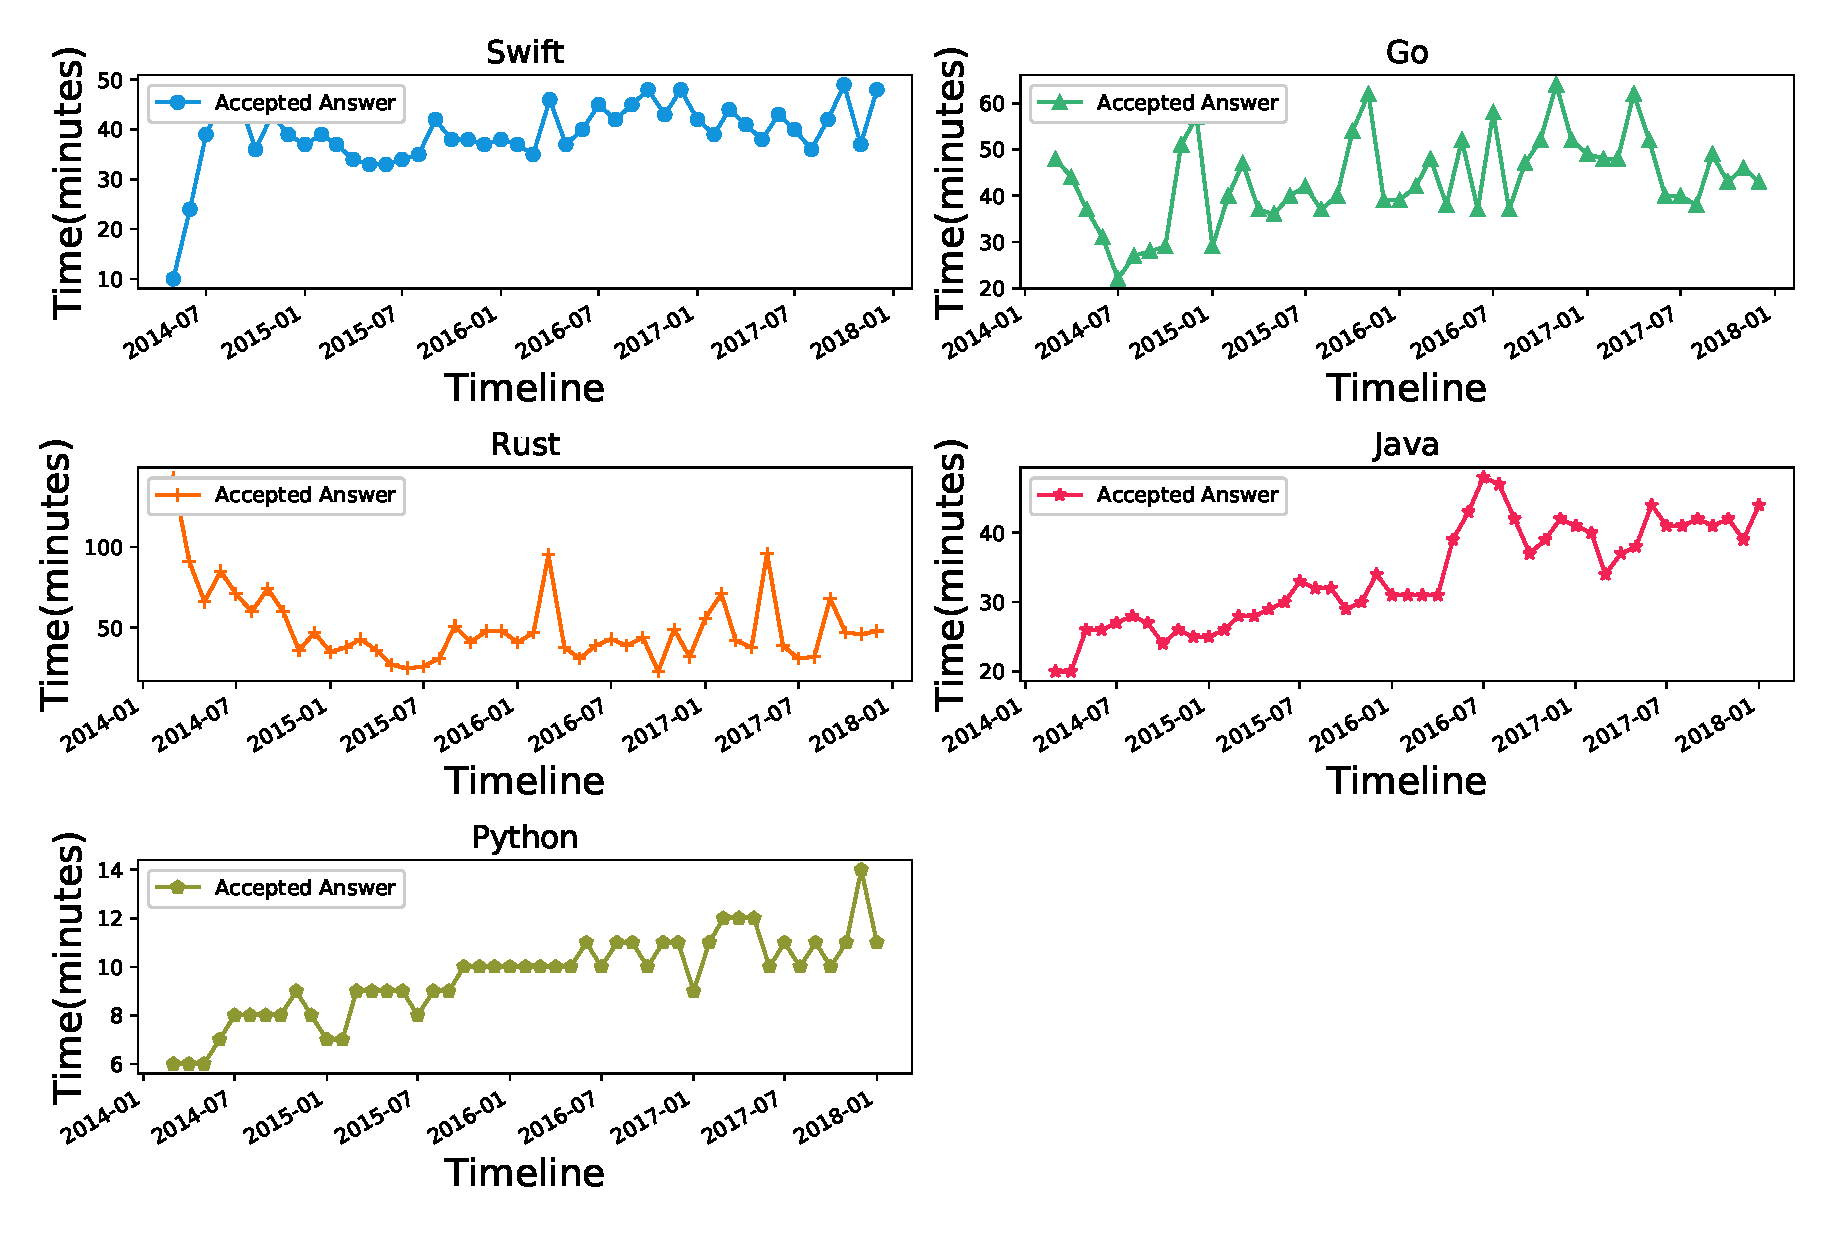
\includegraphics[scale=0.38]{figures/AcceptedAnswerInterval.eps}
\caption{\textbf{Accepted answer}}
\label{fig:Accepted Answer interval}
\end{subfigure}
\begin{subfigure}{0.6\textwidth}
\centering
\hspace{-3cm}
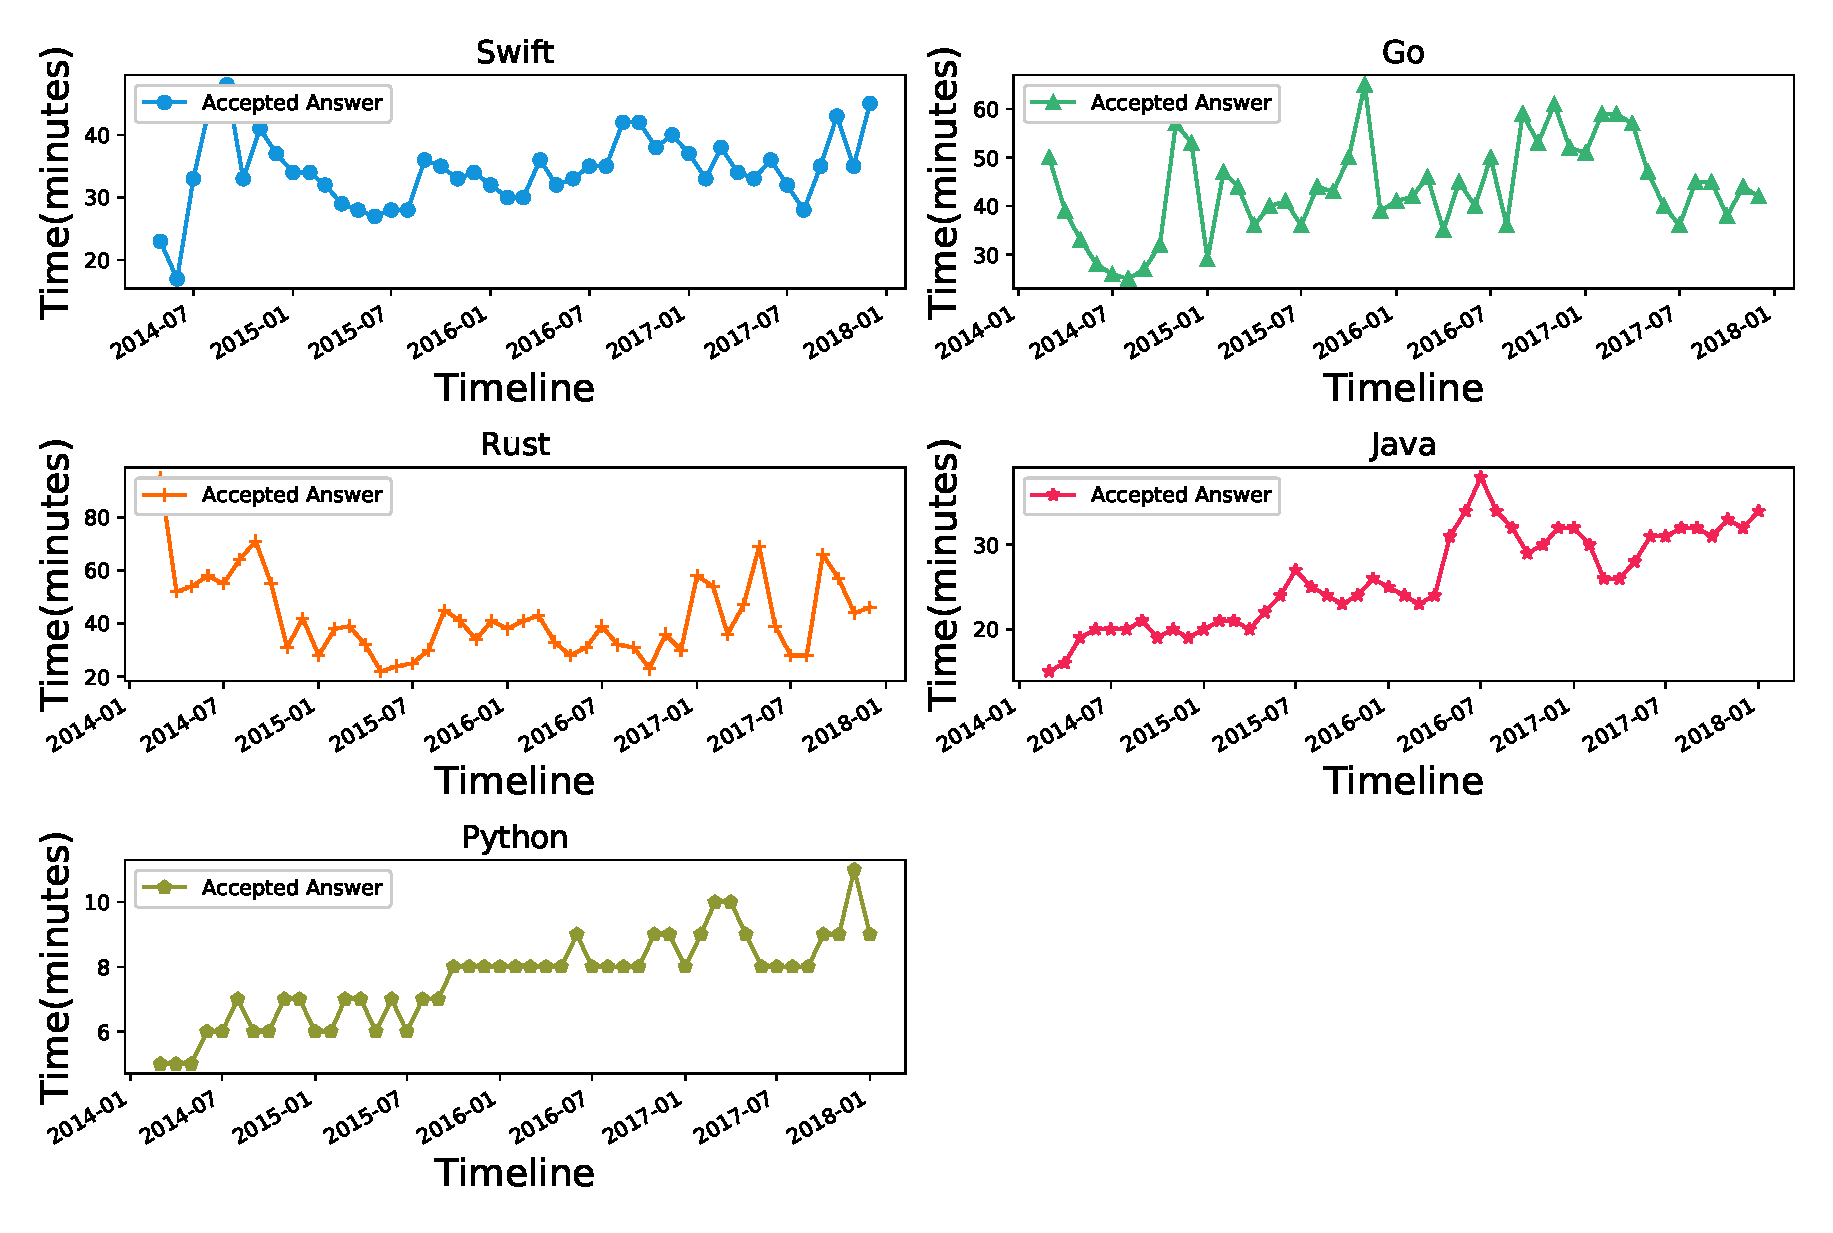
\includegraphics[scale=0.38]{figures/FirstAnswerInterval.eps}
\caption{\textbf{First answer}}
\label{fig:First Answer interval}
\end{subfigure}
\caption{Comparison of median answer interval  of languages in Stack Overflow}
\label{fig:Answer intervals}
\end{figure}
It is assumed that the interval of answers (first and accepted) will be decreased as the language evolves. Figure~\ref{fig:Answer intervals} proves that our assumption is wrong. The answer intervals of Java is increasing in the long run which may be caused by various reason. However, a common reason behind the long answer interval of  stack overflow questions is the inability of that question to attract an expert user to answer that question\citep{Asaduzzaman2013}. However, we can observe steps in the accepted answer interval and the first answer interval of Python and Java. It points out that after a specific time, the answer interval increases. It is common in SO that matured communities often face repeated questions and \emph{hit and run}\citep{DBLP:journals/corr/ChengDL14,SO:decay} problems that cease the necessity of  community collaboration significantly. The increment of answer interval for Python and Java language can be associated with that.
Time to get an accepted answer indirectly represents the growth of developers' expertise. From Figure~\ref{fig:Accepted Answer interval}, it is prominent that Rust has comparatively longer accepted answer interval than the other two new languages. However, it is interesting that this is not true for the first answer interval. Go has longer first answer interval than Rust. Hence, we can say that the accepted answer interval of Rust is longer than Go but Go's first answer interval is longer than Rust. Longer accepted answer interval means the absence of expert developers. Thus, for the Go language, we can claim that Go developers receive the quality answer in the long run, but they have to wait a little longer as active support is absent. That means Stack overflow needs more \emph{active} Go developers and \emph{expert} Rust developers.


\textcolor{green}{To strengthen our claim, we have performed hypothesis testing on accepted answer interval and first answer interval of new languages. To find suitable testing method for hypothesis testing we have performed the Shapiro-Wilk test \citep{SHAPIRO1965}. The Shapiro-Wilk test pointed that the distribution is not normal. Thus we have performed Mann-Whitney U test on first answer interval and accepted answer interval.} The result is presented in Table~\ref{table:accepted-first u value}.
\iffalse
\begin{table}
\centering
%\resizebox{\textwidth}{!}
\caption{Mann-Whitney U test result for the comparison of accepted answer time and first answer time of Go and Rust language}
\label{table:accepted-first u value}
\end{table}
\fi



\begin{table}
\caption{Mann-Whitney U test result for the comparison of accepted answer time and first answer time of Go and Rust language}
\begin{tabular}{|l|c|c|c|}
\hline
\multirow{2}{*}{Test Subject}                                   & \multicolumn{2}{c|}{Language}                                     & \multicolumn{1}{l|}{\multirow{2}{*}{p value}} \\ \cline{2-3}
                                                                & \multicolumn{1}{l|}{Language 1} & \multicolumn{1}{l|}{Language 2} & \multicolumn{1}{l|}{}                         \\ \hline
\multirow{3}{*}{First Answer Interval}                          & Go                              & Swift                           &     0.158                                          \\ \cline{2-4} 
                                                                & Go                              & Rust                            &    \textless 0.01                                           \\ \cline{2-4} 
                                                                & Swift                           & Rust                            &      \textless 0.01                                         \\ \hline
\multicolumn{1}{|c|}{\multirow{3}{*}{Accepted Answer Interval}} & Go                              & Swift                           &        0.389                                       \\ \cline{2-4} 
\multicolumn{1}{|c|}{}                                          & Swift                           & Rust                            &         \textless 0.1                                      \\ \cline{2-4} 
\multicolumn{1}{|c|}{}                                          & Go                           & Rust                            &           \textless 0.01                                    \\ \hline
\end{tabular}

\label{table:accepted-first u value}
\end{table}


From the Table~\ref{table:accepted-first u value}, we can reject the null hypothesis for first answer interval and accepted answer interval of Go-Rust and Swift-Rust pair. It means that the difference between first answer interval and accepted answer interval of Rust-Go and Swift-Rust is statistically significant. It implies that our claim about the first and accepted answer intervals of Go and Rust is true.

\boxtext{\textbf{Finding 7:} In Stack Overflow, it takes significantly higher time to get the first answer in the evolving state than the matured state of a new language.}

\boxtext{\textbf{Finding 8:} In Stack Overflow, we found evidence that Go has comparatively less active community support, and Rust has a small number of expert developers.}

\subsection{RQ5: Predecessor language of interest of the respondents of new languages}
\label{RQ4}
We have confined our search into the predecessor language of interest of the \emph{expert developers}. According to our definition,  \emph{expert developers} are those developers who have answered at least one accepted answer.
To find the predecessor language of interest of the expert developers, we collected all the tags of the questions answered by expert developers and then sorted the tags according to their frequency to get the most frequent tags. The most frequent ten tags for each language is presented in Figure~\ref{fig:dev skills}.
% \begin{table}
\begin{center}
\begin{tabular}{|l|l|}
    \hline
    Developers & Tags in order of occurrence\\ \hline
    
    \multirow{2}{*}{Swift Developers}
    &iOS\\&Java\\&Objective-C\\&Swift\\&JavaScript\\&Android\\&iPhone\\&Php\\&C++\\&C\# \\ \hline
    
    \multirow{2}{*}{Go Developers}
    &Java  \\ &JavaScript\\ &Python \\&C++\\&Php\\&C\#\\&MySQL\\&C\\&Regex\\&JQuery \\ \hline
    
    \multirow{2}{*}{Rust Developers}
    &C++\\&C\\&Java\\&Python \\& Rust\\ &Ruby\\ &C\# \\ &Haskell \\ &JavaScript 	\\ &Linux\\ \hline
    


\end{tabular}
\end{center}
\caption{Most frequent 10 tags answered by expert developers of new languages.}
\label{table:Dev skills}
\end{table}
\begin{figure}[t!]
\centering
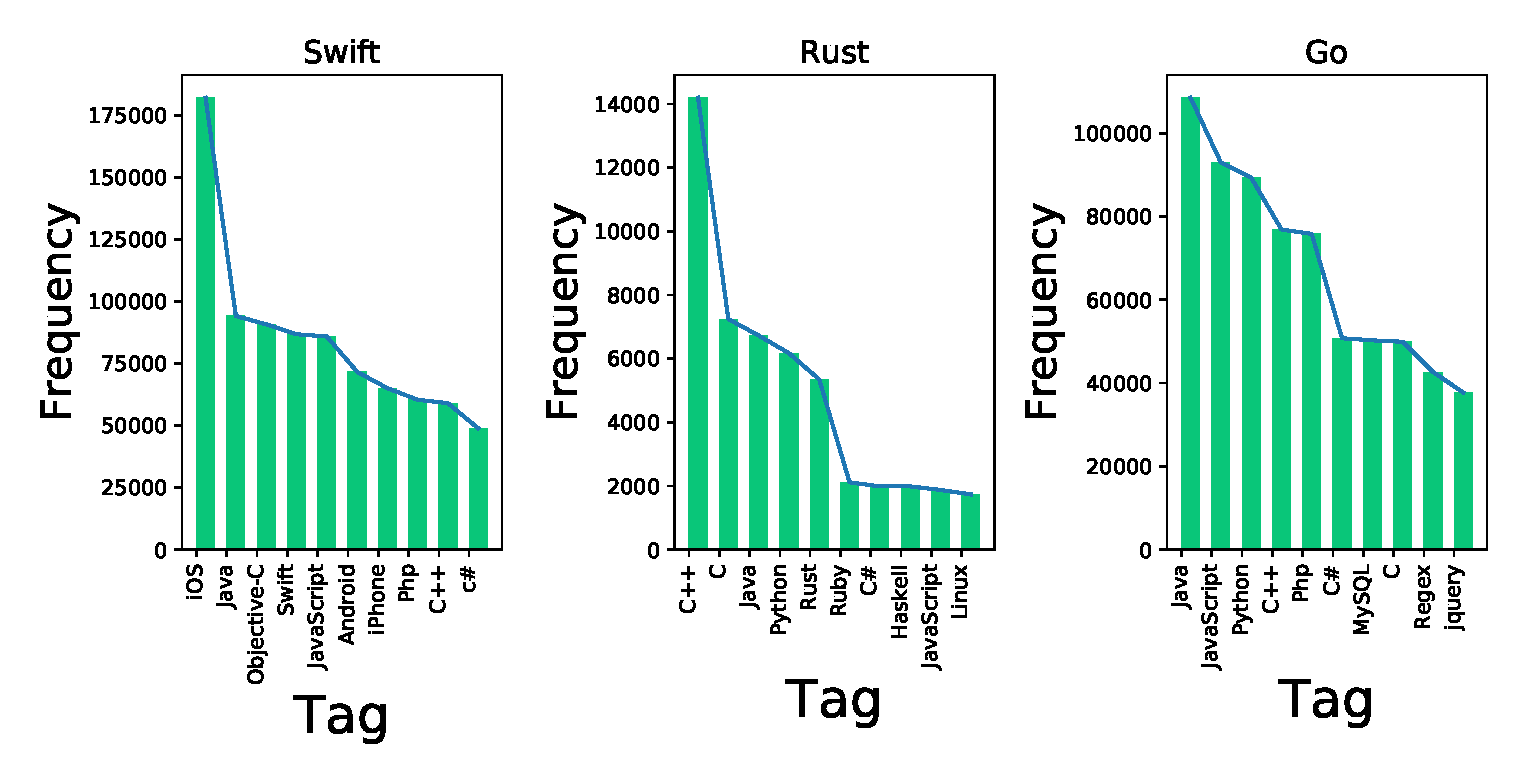
\includegraphics[scale=0.35]{figures/Tagfrequency.eps}
\caption{Most frequent 10 tags answered by expert developers of new languages.}
\label{fig:dev skills}
\end{figure}

Rust experts mostly answered  C and C++ questions. C++ is the predecessor language of Rust. Hence, we can say developers expert in Rust are also expert in C and C++. From that, we can infer that Rust is receiving contributions from the C and C++ community base in Stack Overflow. Developers expert in Swift have mostly answered the Java and Objective-C questions where Objective-C is considered the predecessor of Swift language. Therefore, it is evident that the new languages can get crucial support in their \emph{evolving state} if it has a predecessor language.

\boxtext{\textbf{Finding 9:} New languages are benefited from the community base of the predecessor language.}




\section{Implication}
\label{sec:Implication}
Thus far, we have discussed the characteristics of answer pattern of new languages, the relation between the advancement of new languages and its developers' activity, expected answer interval for new languages, and predecessor language of interest of the respondents of new languages. In this section, we discuss the implications of our findings. As well as helping developers to find resources while learning a new language, our study can also help language owners, researchers, and Stack Overflow to refine their strategies to support the growth of new languages. 

\indent \textbf{Developers:} In this study, we have estimated the answer interval and time when we can expect the availability of the adequate resource in Stack Overflow. If the community support is still evolving in Stack Overflow, then developers can decide to look into other resources. Sometimes community project developed and curated by developers can be an alternative for traditional resources. For example, Rust was a community project of concerned developers. After strong positive feedback, it was donated and has been part of official Rust documentation from Rust 1.25.

\indent \textbf{Language owners:} Our study identifies the significant difference in answer interval between two phases of new languages. As support for the developers in the starting stages is likely to play a significant role in the overall acceptance of that language, owners should provide extensive support during that time. Another option for new languages that are currently in the design stage can be to use the community base of some matured language by carefully selecting predecessor language. Moreover, new languages can try to fill the gap in supporting materials by developer-friendly documentation with detail example. We observed that the issue and release version influences developers' activity pattern(Table~\ref{table:issue_question relationship}, Table~\ref{table:github_question relationship}, Figure~\ref{fig:Release and user behavior}). Though it is not possible to release a bug-free version, extra care must be taken for a bug-free release and solution of issues in GitHub. A good portion of questions in Stack Overflow seeks for clarification of the documentation. Owners should take extra care to prepare documentation suitable for developers of all levels. 

\indent \textbf{Stack Overflow:} Small community size can disrupt the growth of a language. In our study, we have found that the new languages have a small number of experts or active developers in Stack Overflow. To support the growth of a language which has a few expert developers,  Stack Overflow should refine their strategy. According to the current policy, the stack overflow focuses on the expert developers. However, to support new languages, they should encourage developers from all levels to take part in answering questions. It supports the findings of Srba et al.\citep{Srba2016} where they suggested Stack Overflow replace the current question-oriented policy with answer-oriented policy.

\indent \textbf{Researchers:} The topics like parallel execution, mutability, memory allocation are common in the difficult topics of new languages. It proves the limited availability of knowledge in these topics. Researchers may pay attention to these topics as these are an important part of a developer's work practices.

\section{Threats to validity}
\label{sec:validity}
In this section, we discuss the validity of our study.

\indent \textbf{Internal validity:} Use of tags to categorize questions by language is an internal threat to validity. A new Stack Overflow user may not add an appropriate tag with the question. However, Stack Overflow questions go through an extensive moderation process and eventually, it will have the appropriate tags. In some cases, our identification of posts by tags may not be able capture the posts of new languages. To alleviate this threat, we considered the relevance of tags.  In this study, we have used Stack Overflow as the primary dataset. There are many language specific developers' forum and QA sites and it is possible that those sites may contain posts that can help to understand the growth of new languages. However, we believe that a large number of participants and the widespread popularity of Stack Overflow has made it a familiar venue for developers. Hence, the posts of Stack Overflow are considered enough to understand the trends of growth of new language.

\indent \textbf{External validity:} After the inception of the Stack Overflow (2008), about 35 programming languages have been released\citep{wiki:Timeline} whereas this study is focused on three languages (Swift, Go, and Rust). For this reason, our research results may not apply to other new languages. However, in this study, we did not emphasize any specific feature of a particular language. The languages we considered vary in terms of their time of inception and other properties (such as having predecessor language or not). Instead, we focused on the characteristics and trends of the growth of new languages. \textcolor{blue}{We compared the growth trends with top-tier (Java) and mid-category (Python) languages and found that mid-category language (Python) shows similar characteristics. The reason for the dissimilarity with high-level languages is that we missed the community interaction at the initial period of this language. Java was published a long time ago and was already a developed language before the establishment of SO.} Therefore, we think our findings are free from any bias on particular language.

\iffalse

\indent \textbf{Construct validity:} In this study, votes of accepted answers are given double weight in the calculation of post quality. The weight used may not represent their exact contribution. However, the magnitude of weight do not influence our analysis. Thus, double weight in the accepted answer will not invalidate our claim.
\fi
\section{Conclusion}
\label{sec:conclusion}
In this study, we analyze the reflection of the growth of new languages on Stack Overflow, i.e., how the activity pattern of Stack Overflow users changes along with the growth of the resources of the language and the expected time of availability of adequate resources. We show that our findings can help not only developers but also language owners and Stack Overflow to support the growth of new languages. In the early stages of new programming languages, documentation is not very rich and it is likely to be enriched with time. The impact of quality of documentation on the growth of new languages can be a new avenue for our future work. In this study, we have analyzed the reflection of the growth of new languages on Stack Overflow, i.e., how the activity pattern of Stack Overflow users changes along with the growth of the resources of the language, exp. We showed how our findings can help not only developers but also language owners and  Stack Overflow to support the growth of new languages. 




\bibliographystyle{ACM-Reference-Format}

\bibliography{bibliography}

\pagebreak
\appendix
\section{Tags of new languages}
\label{appendix:tagrelevance}
\begin{longtable}{|l|l|l|l|}

\hline
Language                      & $\alpha$ value & $\beta$ value & set of tag \\ \hline
\multirow{24}{*}{Go language}  & 0.01  &  0.02  &  hibernate, mongodb   \\ \cline{2-4}
               & 0.01  &  0.05  &  json   \\ \cline{2-4}
               & 0.02  &  0.01  &  groovy, reflection   \\ \cline{2-4}
               & 0.02  &  0.02  &  http   \\ \cline{2-4}
               & 0.03  &  0.03  &  google-app-engine   \\ \cline{2-4}
               & 0.04  &  0.01  &  interface, google-cloud-datastore   \\ \cline{2-4}
               & 0.04  &  0.02  &  concurrency   \\ \cline{2-4}
               & 0.05  &  0.03  &  struct   \\ \cline{2-4}
               & 0.13  &  0.01  &  grpc   \\ \cline{2-4}
               & 0.13  &  0.1   &  grails   \\ \cline{2-4}
               & 0.15  &  0.01  &  grails-2.0   \\ \cline{2-4}
               & 0.2   &  0.01  &  unmarshalling   \\ \cline{2-4}
               & 0.21  &  0.02  &  slice   \\ \cline{2-4}
               & 0.38  &  0.01  &  grails-domain-class   \\ \cline{2-4}
               & 0.41  &  0.01  &  channel   \\ \cline{2-4}
               & 0.86  &  0.01  &  go-templates   \\ \cline{2-4}
               & 0.91  &  0.01  &  beego   \\ \cline{2-4}
               & 0.97  &  0.01  &  mgo   \\ \cline{2-4}
               & 0.99  &  0.01  &  gorilla   \\ \cline{2-4}
               & 1.0   &  0.01  &  cgo, go-gorm   \\ \cline{2-4}
               & 1.0   &  0.02  &  goroutine   \\ \cline{2-4}
               & 1.0   &  0.1   &  gorm   \\ \cline{2-4}
               & 1.0   &  0.89  &  go   \\ \hline

\multicolumn{4}{|l|}{}                                    \\ \hline
\multirow{25}{*}{Swift language}               & 0.01  &  0.01  &  generics, parse.com, dictionary, cocoa, uiwebview   \\ \cline{2-4}
               & 0.01  &  0.02  &  macos   \\ \cline{2-4}
               & 0.01  &  0.03  &  firebase   \\ \cline{2-4}
               & 0.02  &  0.01  &  \makecell[l]{uiviewcontroller, uiview, uiimageview,\\ uinavigationcontroller, uiscrollview, uiimage}   \\ \cline{2-4}
               & 0.02  &  0.02  &  firebase-realtime-database   \\ \cline{2-4}
               & 0.02  &  0.1  &  xcode   \\ \cline{2-4}
               & 0.03  &  0.01  &  \makecell[l]{uibutton, uitextfield, uilabel, tableview, mapkit,\\ uitabbarcontroller}   \\ \cline{2-4}
               & 0.03  &  0.02  &  core-data   \\ \cline{2-4}
               & 0.03  &  0.06  &  uitableview   \\ \cline{2-4}
               & 0.03  &  0.55  &  ios   \\ \cline{2-4}
               & 0.04  &  0.01  &  realm, cocoapods, avfoundation, segue   \\ \cline{2-4}
               & 0.05  &  0.01  &  protocols, nsuserdefaults   \\ \cline{2-4}
               & 0.05  &  0.02  &  sprite-kit, uicollectionview   \\ \cline{2-4}
               & 0.06  &  0.01  &  swift4, uicollectionviewcell   \\ \cline{2-4}
               & 0.07  &  0.5  &  swift   \\ \cline{2-4}
               & 0.12  &  0.02  &  ios9   \\ \cline{2-4}
               & 0.17  &  0.03  &  alamofire   \\ \hline
               \pagebreak
               \hline
               & 0.21  &  0.03  &  xcode7   \\ \cline{2-4}
               & 0.23  &  0.02  &  ios10   \\ \cline{2-4}
               & 0.39  &  0.06  &  xcode8   \\ \cline{2-4}
               & 1.0  &  0.01  &  \makecell[l]{swift-extensions, swift2.3, swift-package-manager,\\ swift2.1, swift2.2}   \\ \cline{2-4}
               & 1.0  &  0.02  &  swift-protocols   \\ \cline{2-4}
               & 1.0  &  0.03  &  swift-playground   \\ \cline{2-4}
               & 1.0  &  0.29  &  swift2   \\ \cline{2-4}
               & 1.0  &  0.63  &  swift3   \\ \hline
\multicolumn{4}{|l|}{}                                    \\ \hline               
\multirow{25}{*}{Rust language} & 0.01  &  0.01  &  types, reference, enums, pattern-matching, hashmap   \\ \cline{2-4}
               & 0.01  &  0.02  &  vector, struct   \\ \cline{2-4}
               & 0.01  &  0.03  &  generics   \\ \cline{2-4}
               & 0.02  &  0.01  &  slice   \\ \cline{2-4}
               & 0.02  &  0.02  &  iterator, macros   \\ \cline{2-4}
               & 0.03  &  0.01  &  future   \\ \cline{2-4}
               & 0.03  &  0.02  &  closures   \\ \cline{2-4}
               & 0.07  &  0.01  &  mutable   \\ \cline{2-4}
               & 0.21  &  0.02  &  ffi   \\ \cline{2-4}
               & 0.24  &  0.04  &  traits   \\ \cline{2-4}
               & 0.3  &  0.01  &  ownership   \\ \cline{2-4}
               & 0.66  &  0.06  &  lifetime   \\ \cline{2-4}
               & 0.87  &  0.01  &  hyper   \\ \cline{2-4}
               & 1.0  &  0.01  &  serde, borrowing, rust-tokio, rust-crates   \\ \cline{2-4}
               & 1.0  &  0.03  &  borrow-checker   \\ \cline{2-4}
               & 1.0  &  0.04  &  rust-cargo   \\ \cline{2-4}
               & 1.0  &  1.0  &  rust   \\ \hline
               
               
\caption{Significant and relevant tags of new languages used  to identify posts of new languages.}
\end{longtable}


\section{Topic listings}
\label{appendix:LDA topic}
% Please add the following required packages to your document preamble:
% \usepackage{multirow}
{\color{green}
\begin{longtable}{|l|l|l|}
% \begin{tabular}{|l|l|l|}

\hline
Language              & Topic name & Top LDA words  \\ \hline
\multirow{6}{*}{Go}   & Problem in using library           & \textit{\begin{tabular}[c]{@{}l@{}}hql, gorm, mgo, grail,  dgo, beego,\\ hikari, error\_handling, groovy\end{tabular}}\\\cline{2-3}

                      & Serving request                    & \textit{\begin{tabular}[c]{@{}l@{}}grpc, server, ip\_address,\\request, testing, protocol,\\ socket, unmarshal, encryption\end{tabular}}\\\cline{2-3}
                      
                      & Go channel                         &  \textit{\begin{tabular}[c]{@{}l@{}}testing,
                      channel, mutex, thread,\\ http, syntax, lock, goroutine,\\ concurrency\end{tabular}} \\\cline{2-3}
                      
                      & Compilation problem                & \textit{\begin{tabular}[c]{@{}l@{}}gcompiler, go\_build, dwarf, cgo,\\ signed, flags, goreleaser, gocache, CI \end{tabular}}\\\cline{2-3}
                      
                      & Memory                             &   \textit{\begin{tabular}[c]{@{}l@{}}slice, memory\_allocation, network, io,\\ buffer, marshall, memory\_leak, pointer,\\ allocation\end{tabular}}\\\cline{2-3}
                      
                      & Migration Problem                  & \textit{\begin{tabular}[c]{@{}l@{}}data\_structure, server\_tech, language\_ equivalent,\\ compiler, syntax, clang integration,\\ convert, client\_communication, cgo\end{tabular}} \\\hline
\multirow{6}{*}{Rust} & Use of Struct        & \textit{\begin{tabular}[c]{@{}l@{}}syntax, lifetime,                                type\_conversion, algorithm,\\ clone, enclosed, filter, reference,\\                                           initialize\end{tabular}}\\\cline{2-3}

                      & Mutability           &  \textit{\begin{tabular}[c]{@{}l@{}}mutability, dref, scope,\\ moved\_value, closure, immutable,\\ FnMut\end{tabular}}\\\cline{2-3} 
                      
                      & Parallel execution   &  \textit{\begin{tabular}[c]{@{}l@{}}threads, sync, channel, rayon,\\ thread\_join, prelude, sequential, faster\end{tabular}}\\\cline{2-3}
                      
                      & Borrow mechanism     & \textit{\begin{tabular}[c]{@{}l@{}}borrow, frozen\_variable, ref, lifetime,\\ shadow, overlap, move, reuse, access\end{tabular}}\\\cline{2-3}
                      
                      & Use of Trait         & \textit{\begin{tabular}[c]{@{}l@{}}trait, static, dynamic, pointer,\\ polymorphism, unbox, generic, concrete,\\ conflict \end{tabular}}\\\cline{2-3}             
                      & Migration problem    & \textit{\begin{tabular}[c]{@{}l@{}}equivalent, compiler, syntax, jni,\\ extern, convert, pass, FFI,\\ wrap \end{tabular}}               \\\hline
\multirow{6}{*}{Swift}& UI                           &\textit{\begin{tabular}[c]{@{}l@{}}Ui,                                       view\_controller, animation,\\ layout, swiftUI, segue, graphics,\\ sprite, scene\_kit                           \end{tabular}}\\\cline{2-3}

                      & View Controller lifecycle    &\textit{\begin{tabular}[c]{@{}l@{}}hooks, cg\_size, appear,\\ disappear, will\_appear, deinit,\\ view, timer, dynamic \end{tabular}}\\\cline{2-3}
                      
                      & Mutability                   &\textit{\begin{tabular}[c]{@{}l@{}}collection, mutation, struct, let,\\ reference, mutable, modify, pointer,\\ unsafe\end{tabular}}\\\cline{2-3}
                      
                      & Data Handling                &\textit{\begin{tabular}[c]{@{}l@{}}database, json, parsing, persistence,\\ keychain, coredata, types, optional,\\ nested\end{tabular}}\\\cline{2-3}
                      
                      & Migration problem            &\textit{\begin{tabular}[c]{@{}l@{}}nullability, header, sub\_class,\\ swiftify , bridging, equivalence, object\_conversion,\\ protocol, dependency\end{tabular}}\\\cline{2-3}
                      
                      & Documentation clarification  &\textit{\begin{tabular}[c]{@{}l@{}}syntax, documentation, pragma\_mark,\\ xcode, comments, sdk, reference,\\ tutorial, apple-documentation\end{tabular}}\\\hline

         
% \end{tabular}
\caption{Topics discovered by LDA}
\end{longtable}}
    
\end{document}